\documentclass[11pt,twoside]{book}
\usepackage[a4paper,top=0.9in, bottom=2.54cm, vscale=1,inner=3.5cm,outer=2cm]{geometry}
\usepackage{setspace}
\onehalfspacing
\usepackage{subcaption}
%\usepackage[doucument]{ragged2e}
%\raggedright
\usepackage[british]{babel}
\usepackage[utf8]{inputenc}
\usepackage{amsmath}
\usepackage{graphicx}
\usepackage{parskip}
%\usepackage{natbib}
\usepackage{pgfgantt}
\usepackage{lscape}
\usepackage{tabularx}
\usepackage{pdfpages}
\usepackage{graphicx}
\usepackage{xcolor}
\usepackage[listingsutf8,minted]{tcolorbox}
\usepackage{hyperref}
\usepackage[chapter]{tocbibind}
\usepackage{doc}
\usepackage{minted}
\usepackage{listings}
\usepackage{listingsutf8}
\usepackage[colorinlistoftodos]{todonotes}
\usepackage{float}
\usepackage{lastpage}
\usepackage{wrapfig}
\usepackage{filecontents}
\usepackage{amsmath}
\usepackage{mleftright}
\newcommand{\lnn}[1]{%
  \ln\left(#1\right)%
}

\newcommand{\lnb}[1]{%
  \ln\mleft(#1\mright)%
}
%New colors defined below
\definecolor{codegreen}{rgb}{0,0.6,0}
\definecolor{codegray}{rgb}{0.5,0.5,0.5}
\definecolor{codepurple}{rgb}{0.58,0,0.82}
\definecolor{backcolour}{rgb}{0.95,0.95,0.92}

%Code listing style named "mystyle"
\lstdefinestyle{mystyle}{
  backgroundcolor=\color{backcolour},   commentstyle=\color{codegreen},
  keywordstyle=\color{magenta},
  numberstyle=\tiny\color{codegray},
  stringstyle=\color{codepurple},
  basicstyle=\ttfamily\footnotesize,
  breakatwhitespace=false,         
  breaklines=true,                 
  captionpos=b,                    
  keepspaces=true,                 
  numbers=left,                    
  numbersep=5pt,                  
  showspaces=false,                
  showstringspaces=false,
  showtabs=false,                  
  tabsize=3
}

%"mystyle" code listing set
\lstset{style=mystyle}

\usepackage{enumitem}
%\usepackage[]{biblatex}
\usepackage[style=authoryear-ibid,backend=biber]{biblatex}
\addbibresource{writing.bib}
\usepackage{fancyhdr}
\pagestyle{fancy}
\fancyhead{}
\fancyhead[RO,LE]{}
\fancyfoot{}
\fancyfoot[LE,RO]{\thepage \hspace{0cm} of \pageref{LastPage}}
\fancyfoot[LO,CE]{Chapter \thechapter}
\fancyfoot[CO,RE]{16018262}
\usepackage{etoolbox}
\patchcmd{\chapter}{\thispagestyle{plain}}{\thispagestyle{fancy}}{}{}
\begin{document}

\frontmatter
%!TeX root=Dissertation.tex

\begin{titlepage}
\Large
A Report submitted in partial fulfilment of\\
 the regulations governing the award of
\par
the Degree of\\[5mm]
{\huge	 BSc (Honours) Computer Science }\\[5mm]
at the University of Northumbria at Newcastle
\par
\vspace*{1in}
{\Large Project Report}
\par\vspace{1em}
%{\Huge Using website log files to detect low bandwidth attacks through the application of heuristic analysis}
{\Huge A Formulaic approach of detecting website attack traffic with critical evaluation of current methodology}
\vfill
Peter Smith
\par\vspace{1em}
2019 / 2020
\par\vspace{1em}
Software Engineering Project
\par\vspace{1em}
SUPERVISOR: Nick Dalton
\par
2\textsuperscript{\small nd} Marker: Neil Eliot
\end{titlepage}

%!TeX root=Dissertation.tex
\chapter{Declaration}
(1) that the material contained in this dissertation is the end result of my own work and that due acknowledgement has been given in the bibliography and references to ALL sources be they printed, electronic or personal.

(2) the Word Count of this Dissertation is 24810

(3) that unless this dissertation has been confirmed as confidential, I agree to an entire electronic copy or sections of the dissertation to being placed on the eLearning Portal (Blackboard), if deemed appropriate, to allow future students the opportunity to see examples of past dissertations. I understand that if displayed on eLearning Portal it would be made available for no longer than five years and that students would be able to print off copies or download.  

(4) I agree to my dissertation being submitted to a plagiarism detection service, where it will be stored in a database and compared against work submitted from this or any other School or from other institutions using the service.  

In the event of the service detecting a high degree of similarity between content within the service this will be reported back to my supervisor and second marker, who may decide to undertake further investigation that may ultimately lead to disciplinary actions, should instances of plagiarism be detected.

(5) I have read the Northumbria University/Engineering and Environment Policy Statement on Ethics in Research and Consultancy and I confirm that ethical issues have been considered, evaluated and appropriately addressed in this research.
 


%!TeX root=Dissertation.tex

\chapter{Acknowledgements}

I would like to thank my supervisor Nick Dalton for his continual support and guidance during
the project. Nick has been a great source of
advice and direction for me over the past year and for this I thank him greatly.

I would also like to thank all of my support workers; Darren, Garry and Nathan who have enabled me in writing this thesis.

I would like to express my thanks to Graham Baty who kindly offered his support in proof reading this work.

I would also like to thank the producers of the \citeauthor{javaloc} GeoIP database and Java API is used in this  project  distributed under the Creative Commons Attribution-ShareAlike 4.0 International License (\url{https://creativecommons.org/licenses/by-sa/4.0/}) it allows for use and redistribution the material in any medium or format. It is used as part of this project so an IP can be located and given a risk.



Finally, I would also like to take this opportunity to thank my parents for
their continued support and patience for the past three years.



















%!TeX root=Dissertation.tex

\chapter{Abstract}

This thesis identifies that there is a general lack of research into low bandwidth attacks, and there are many inherent difficulties in detecting instances of such attacks. Much of the previously available literature proposed methods for detecting low rate attacks that contained certain fundamental flaws. Many of these methods were not built with scaling in mind and would be unable to function on servers that run more than one website. The main focus of this research was to create a new approach to low rate bandwidth detection that can function at a website admin level.

This work looks at data over a long period of time and is therefore better to identify malicious traffic, specifically when looking at low rate bandwidth attacks. The methodologies that are published online have several weaknesses and therefore are not applicable. No literature could be found during this study, looking at the effects of having multiple websites on a server and the ability to detect attacks on a single website, thus, the implementation of such technologies are needed. The details pertaining to their flaws will be discussed elsewhere in this paper.

This thesis reviews a range of modern detection techniques in order to better understand potential flags for malicious low rate activity. Literature reviewing fully automated and human moderated system approaches has been reviewed in order to assess the best results in detection accuracy. A methodology for detecting low rate bandwidth attacks has been structured using a formulaic principal that reads log files and interprets the risk factor of incoming traffic. The literature review revealed a number of usability issues when creating a user interface for malicious detection, in particular when novice users are involved. In order to combat this, a simple user interface was created to work hand in hand with the software that was designed with novice users in mind. A human moderator, even with little or no Cyber security knowledge, can interpret the data from the software and root out any rare errors or false alarms generated by the formula.

The results were conclusive with a good accuracy in detecting low rate bandwidth attacks from a limited data set. The software that was created as a part of this research has little or no effect on computational resource on a target website. The testing, as part of this research, assessed a one month period of log file activity across 3 websites. The results returned a particularly low margin of error for false alerts. As mentioned, a human moderator with access to the log file data would eliminate the few false alerts generated by the system.

\tableofcontents
\listoffigures
\mainmatter
\chapter{Introduction}

As mankind heads into the twenty first century, the internet has become a critical part of the infrastructure for everyday life. As such, it has developed into a vital economic asset for every country. Many aspects of modern society are now switching towards the use of internet, either partially or exclusively. This creates a delicate check in the vein which can be exploited by bad actors, such as malicious foreign governments or criminal organisations, looking to deny availability to websites for ransom or political gain. An infamous example of an attack for political gain was carried out during the UK general election of 2019. The Labour Party was hit by a two stage cyber-attack that attempted to cripple their website during this critical time (\cite{Labour}). Labour commented that these attacks originated from computers in Russia and Brazil and attempted to flood their servers with illegitimate traffic. Fortunately many of the affects of the attacks were mitigated by their use of Cloudflare's defensive mechanisms, which shall be discussed in depth during this thesis.


As the internet grows and becomes increasingly more reliant upon richer content, through social media and video, it has become apparent that HTTP/1.1 is becoming outdated and substandard to functionality.Its replacement, HTTP/2 was found to have a host of security limitations, which will be discussed later on in this thesis. Due to the widespread adoption of HTTP/2 over the last couple of years as a replacement for HTTP/1, research needs to be conducted into the safety of HTTP/2, the conclusions from the 2016 study by Erwin Adi suggested that the HTTP/2 protocol does not restrict the intensity of traffic generated. This highlighted the need for further research into the protocol itself. A potential application of a further protocol or mechanism with the aim of identifying the volumes and patterns of network traffic communicated between a client and network machine may be required. After consideration of the conclusions from the Erwin Adi studies it was decided to investigate the potential of creating an early detection methodology. A consideration of using the HTTP/2 format here is that during the writing of this report HTTP 3 became available to a limited number of websites, however, due to how new this protocol is, there is a lack of research available in order to assess the protocol within this work.


Due to the ability to automate these malicious assaults, it is not just large organisations that need to feel the danger of attacks. These high rate bandwidth attacks overload the server with false communication, hence denying it to legitimate users by what is known as a denial of service attack (DoS). A report from NETSCOUT has estimated that Distributed Denial of Server (DDoS) attacks alone could be costing the UK economy more than £1 billion a year due to the damage being done. The report estimated that the average cost for each UK business that had seen downtime due to DDoS attacks exceeded £140,000 (\cite{Costs}).

The use of real time attack prevention software such as that offered by Cloudflare is widely accepted and used by businesses and organisations. There is an abundance of software that is available at a commercial level for high rate bandwidth protection. This thesis evaluates why high rate DoS attacks are easier to detect and mitigate, however, these are normally used by large scale hosting providers and other content delivery network providers. Whilst these are normally very effective at blocking such attacks, there are some inherent flaws with these types of protection methods. 

\section{Topic of Research}

This research looks at some of these industrial approaches to current protection methodology, however, the research also considers past studies into the methodology of detection for Low rate and port scanning attacks. High rate bandwidth attacks are reviewed with regards to the ease of identification, and identify the reasons why. A critical evaluation of current and historical techniques has been conducted in order to establish an outline for best practice in attack detection. It was the the directive of the research to create a formulaic program to assess the risk of incoming traffic, that is resource effective and user friendly. The planned architecture of the formula was purposed to be able to accurately identify a variety of attacks. The formula also needed to be generic enough to be used on a variety of websites.

The first is that these systems mainly rely on real-time data and traffic; this data is aggregated, therefore, what may be an attack on one website could potentially not be flagged on another. This is because, to the overall network, what looks like a normal traffic pattern on one website may in fact be malicious on another, due to the aggregated nature of the data. Current systems do not provide a lot of information to the end users; this may increase the risk factor to their website making it less safe and giving them a less accurate picture of what is going on. For example, they may see more traffic than normal, however, they may not be informed if there is a legitimate traffic spike or a malicious attack. An attack may be stopped; this may make the website owner complacent in regards to security. The software proposed will try to actively engage the users in their security.

The research had theorised that the data contained within log files would be sufficient to diagnose malicious trends of incoming traffic. As the information stored within the log files is particularly meagre, the research has attempted to utilise as many aspects as possible from the raw data to draw conclusions regarding risk related elements. After studying the log file data in greater depth, the risk factors have been given a scoring system in order to formulate a mathematical approach to aid in the detection of malicious traffic. 

As it could be the case that this software might be used by individuals with limited PC awareness, this thesis also consults historical studies into human computer interaction. In particular this work looks at the ability of non-cyber security experts in identifying attacks. With this knowledge, an appropriate user interface has been constructed with the principle of working hand in hand with the software to identity low-rate bandwidth attacks. The lack of concrete research on Low-bandwidth attacks that are able to work in a production environment is a concern to the safety of those on the internet, therefore, this work will propose new ways of detecting attacks that are able to work in a production environment.

\section{Scope of Work}

It is important to set out the framework of the scope of research in terms of what is deemed to be achievable within the window of the project. It is the intention of the thesis to build a system for identifying and mitigating malicious traffic. This may include a mixture of a formulaic approach, AI or a human moderator. After the literature review is conducted, best practices in methodology shall be adopted using the lessons learned by prior researchers into the field.

Due to the varying nature of attacks that can take place online, particularly on a website, any formula or AI proposed for construction in this thesis shall be limited to the detection of common attacks. The system shall take a 'broad stroke' approach to detection methodology. However, it is theorised that attackers are using a constantly evolving stealth strategy. Therefore it is reasonable to conclude that the software may not be able to detect every type of attack with a high degree of accuracy.

A user interface shall be designed to work hand in hand with the developed software. Whether or not this user interface is purely intended to run the program, or used in the process of threat detection, user testing shall be carried out to promote ease of use and user understanding. Although the user interface shall be functional and practical, it is not the intention to produce a user interface suitable for commercial release. This may mean that the user interface will be less visually impressive than standards expected for a marketable product.

\chapter{Review of current detection methods for low bandwidth attacks}
\section*{Introduction}
This chapter will look at available literature that focuses on various types of attacks that require low amounts of bandwidth. As part of this section, port scanning attacks will also be addressed and studied with supporting literature. In general these types of attack are much more difficult to detect that high bandwidth attacks, and an evolving strategy of stealth has been adopted by attackers over the years. It should be noted that port scanning attacks in general could be broken down into many different sub categories. A detailed breakdown of these subcategories shall be presented in section 2.2.1. Due to the fundamental core architecture of port scanning attacks, the literature review shall cover the attack definition as a whole, rather than addressing each subcategory.

In order to approach the topic of low rate and port scanning attacks some basic understanding of terminology should be addressed. In general these types of attack rely upon a weaknesses in protocol such as the transmission control protocol (TCP). A TCP is a connection-oriented protocol, a connection needs to be established before two devices can communicate. TCP uses a process called three-way handshake to negotiate the sequence and acknowledgment fields and start the session. Two devices would be in communication, the Client and the Server. The Client initiates the connection by sending the TCP SYN (SYNchronize) packet to the destination Server and the Server receives the packet and responds with an acknowledgement. The Client then acknowledges the response of the Server by sending the acknowledgment back, and a connection is formed. 
It is also important to understand the current web-server protocols and their differences in terms of security. It is the initial assumption that there are differing vulnerabilities for HHTP/2 and HTTP/1.1 web-servers. HTTP/2 (defined as RFC 7540), is a more modern protocol, than that of HTTP/1.1 (defined as RFC 2616). It is assumed that due to the recent implementation of this protocol that it has more vulnerabilities through a wider range of threat vectors. This shall be investigated and hopefully illustrated through the literature available for study in this chapter. The initial ideology behind this theory was formed when, Tripathi suggested that HTTP/2 has more threat vectors than HTTP/1.1 (\cite{tripathi2018slow}). Adi also notes that "The HTTP/2-standard states that if the host machine does not monitor resource usage, it exposes itself to the risk of a DoS attack" (\cite{Adi2015}).

The comprehension of these protocols are key in the greater understanding of how both low rate bandwidth attacks and port scanning attacks operate. Both of these attacks will actively exploit protocols to carry out their attack. 
%!TeX root=Dissertation.tex

\section{Low-bandwidth attacks} \label{attack1}

A low and slow attack is a type of DoS or DDoS attack that relies on a small stream of very slow traffic which can target application or server resources. A DoS attack is a denial of service attack where a computer (or computers) is used to flood a server with TCP and UDP packets. A DDoS attack is where multiple systems target a single system with a DoS attack. The targeted network is then bombarded with packets from multiple locations. Unlike more traditional brute-force attacks, low and slow attacks require very little bandwidth and can be hard to mitigate, as they generate traffic that is very difficult to distinguish from general traffic. Because they don’t require a lot of resources to pull off, low and slow attacks can be successfully launched using a single computer. In comparison, a high rate attack is launched from numerous compromised devices, often distributed globally in what is referred to as a botnet. A botnet refers to a group of computers which have been infected by malware and have come under the control of a malicious actor. It is distinct from low rate attacks, in that it uses a single Internet-connected device (one network connection) to flood a target with malicious traffic. 


Low rate and low bandwidth attacks differ greatly from a high rate DoS attack (High bandwidth attacks shall be discussed in depth in Chapter 3). A DoS attack, works on overwhelming the server with requests, therefore, it is easier to detect than a low-rate attack. An example of this would be if you were to receive a large amount of traffic from a single IP; this more than likely would be a DoS attack. A normal internet request operates based on an HTTP GET request to the web server that allows access to the site, the outcome of a DoS attack is the creation of a disruption between the clients and the web host. 

High-bandwidth attacks will keep trying to request multiple web pages at the same time to overwhelm the server. In comparison, a low-bandwidth attack  will send a partial request and may wait 20-30 seconds, it then sends new data, just enough to keep the connection open. One type of a Low-bandwidth attack is a slow loris attack; this is a layer-7 application attack, that only requires a small level of band-width and thus means the attacker can have continual use over their system and carry out normal activity. A web server will have a set number of sockets that it can have open at any one time, for this explanation we will choose to use 10 sockets. The aim of a slow loris is to open all 10 sockets and keep them busy, therefore, no new sockets can be opened and thus, no client interaction will take place. The difficulty with detecting these types of attacks is that the legitimate user may just have a slow internet connection, thus making it difficult to distinguish these attacks from slow users. 

%!TeX root=Dissertation.tex
\subsection{Attack Detection Techniques}

The largest amount of research done into low rate Dos attacks is by \citeauthor{Adi2015}. His team's work started in 2015 and they have 3 papers on this subject, the last of which was written in 2018. The majority of their work looked at using resource utilisation in order to detect low bandwidth attacks. They set numerous tests to analyse the behaviours of victim machines when subjected to low rate Dos Attacks. 

The 2016 study carried out four varying investigations to analyse the behaviour of a victim machine when subjected to large volume low rate DoS attacks. The researchers used a flood of windows PING and WINDOWS UPDATE frames to Simulate a Low-Rate DoS attack on a server, and demonstrated legitimate HTTP/2 high volume traffic (flash Crowd) could be launched to create a DoS scenario. The team noted at the time of their 2016 investigation that there was no reported study to ascertain whether or not attack traffic could be concealed in a stealthy manner to appear as legitimate flashcrowd traffic. The research concluded that the HTTP/2 protocol itself does not restrict the intensity of traffic generated, and that auxiliary mechanisms should be implemented for identifying volumes and patterns of network traffic 
\begin{wrapfigure}{R}{}
\label{addie table}
    \centering
    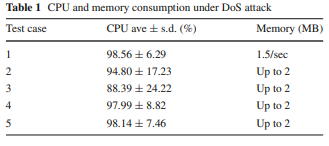
\includegraphics{Apdenix/adiTable.PNG}
    \caption{Table 1 from \citeauthor{adi2017stealthy} \citeyear{adi2017stealthy}}
    \label{fig:my_label}
\end{wrapfigure} (\cite{Adi2016}). Tripathi stated as criticism in his 2018 study that neither the 2015 or 2016 studies completed by Adi's team managed to achieve a completed exhaustion of computational resource (\cite{tripathi2018slow}). Therefore it could be argued that Adi's research did not represent the full effect of a DoS attack. When looking into the details of the results from Adi's research, the figures quoted in Table 1 (Figure 2.1) in the paper by Adi show depletion rates of between 88.39\% to 98.56\% (\cite{Adi2016}).

Due to the ineffective depletion of the CPU the majority of Adi's detection methods could be questioned. Erwin Adi himself points out that his methodology could potentially be flawed due to the reduction of resource status that was achieved. Therefore Adi's proposed method for monitoring CPU depletion as a way to detect low rate bandwidth attacks could be fundamentally in-concise. Adi's study was completed on a server with one single website and did not run any other background services for example, email, which would in theory add unpredictable CPU loads and make his detection method difficult to implement.


\begin{wrapfigure}{L}{}
\label{web using h2}
    \centering
    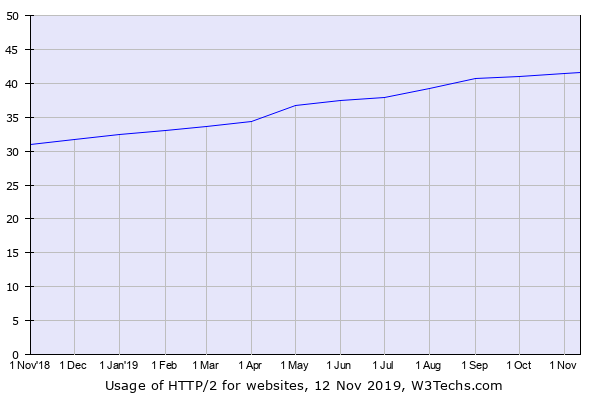
\includegraphics[width=88mm,scale=0.8]{Apdenix/HTTP2SITESgraph.png}
    \caption{Usage of HTTP/2 for Websites, 12 Nov 2019, W3Techs.com}
    \label{web http2}
\end{wrapfigure}
Although Adi's 2016 work looked at HTTP/2 it was noted in their later 2017 paper that 90\% of contemporary web servers up to the date of that study had not yet migrated to HTTP/2 from HTTP/1.x (\cite{adi2017stealthy}) At the time of this thesis, November 2019, HTTP/2 was used by 41.7\% of the top 10 million websites (\cite{w3techs}), as seen in figure \ref{web http2}. This illuminates the pressing need for research into the safety of the HTTP/2 protocol and consequent detection methods and fixes. 
 
Tripathi's 2018 study took a sample of websites and attempted to detect low rate attacks by monitoring benchmarking and measuring the Chi squared (X\textsuperscript{\small2}) differential value between the expected and observed traffic pattern. Tripathi suggests this approach could detect attacks with high accuracy and may lead to future research to assess further HTTP/2 vulnerabilities, thus potentially mitigating these threat vectors with fixes. Tripathi indicated that although his detection method for attack traffic was successful; if HTTP/2 traffic data is encrypted it must then be decrypted before submitting traces to the detector. He suggested that this could be easily achieved with the aid of an intercepting proxy before forwarding to the target website responsible for handling HTTP/2 requests. It must be noted that most large companies are utilising this strategy to intercept traffic coming into their local network. (\cite{tripathi2018slow}). 

Adi's 2017 work looked at some of the stealthier approaches that cyber attacks were using in order to bypass current detection methods. Adi and his team set up two models intended to simulate stealthy low rate DoS attacks which they called 'bots'. The investigation aimed to model attacks whose traffic continually consumed the victims computing resource, while still being stealthy enough to yield some false alarms via the target servers' 'learning' mechanisms. Adi constructed the attack 'bots' with four core factors for experimentation, these were number of threads, number of window\_update, stealthy factors and the delay between successive TCP connections. These two sets of Stealth models were tested against regular flash crowd traffic in an effort to differentiate the pattern. The experiment and subsequent analysis was successful in distinguishing a notable difference in the patterns of the number of packets carrying SYN flags per 1-second traffic instance between regular flashcrowd traffic and the simulated stealthy attacks (\cite{adi2017stealthy}). Since Adi's work there appears to be an implementation of the methodology proposed in their paper. For example, Cloudflare have been able to implement a defence mechanism against a SYN flood attack. The have created a program called 'gatebot' which monitors SYN packet requests and attempts to drop malicious SYN packets on the firewall layer (\cite{CFSYN}) the work does not refer to that of Adi's however the Cloudflare implementation does appear to use similar concepts. At the  time of writing this seems to be the only documented attempt of blocking SYN attacks.

This section has highlighted the lack of research and mitigation of low rate bandwidth attacks which can easily occur and disrupt a website whilst going undetected.
%!TeX root=Dissertation.tex
\section{Port scanning}
Port scanning is an attack whereby a malicious user will send packages of information to different ports on a server to see which ports can be accessed. These types of probe attacks are not expected to be harmful on their own, however, they can be a prelude to a further more serious attack such as a brute force attack. It is important to note that the purpose of ports is varied and some ports expect a much higher volume of traffic than others. For example: Port 80 (unencrypted) and 443 (encrypted), deal with website traffic and are generally expected to be heavily used. A popular scan target for attackers is the SSH 22 port which is essentially a gateway to an entire network. An open SSH port can result in a probe attack being followed up with a hostile attempt to take control of the network. A lot of web hosts and server owners change the ports for SSH and the ftp ports to make it harder to access them, however, they may inadvertently leave ports open that are not secure. It is important to note that all port scanning attacks utilize the TCP 'three way handshake' that was explained in the previous section. (\ref{attack1})
%https://ieeexplore.ieee.org/stamp/stamp.jsp?tp=&arnumber=6122824
\subsection{Different types of Port Scanning Attacks}

After reading the literature regarding the various attacks, the types of port scanning attacks can be condensed down to the 5 following categories:
\begin{itemize}
    \item Ping Scan
    \begin{itemize}
        \item The method of ping scanning entails sweeping an entire network block or a single target, to asses if the target is live. It sends an ICMP echo request to the target, and if the response is an ICMP reply, then you know the target is alive. It is becoming increasingly common that ICMP pings are being blocked by firewalls and routers, that this attack method is becoming ever more ineffective.
    \end{itemize}
    \item TCP Half-Open
    \begin{itemize}
        \item This is probably the most common type of port scan. This is a relatively quick scan that can potentially scan thousands of ports per second. It works this way because it does not complete the TCP handshake process that was discussed in section \ref{attack1} of this chapter. It simply sends a packet with the SYN flag set and waits for the SYN-ACK from the target and does not complete the connection. After identifying open ports the attacker may then escalate this probe with a further attack, for example a brute force attack against an open port.
    \end{itemize} 
    \item TCP Connect
    \begin{itemize}
        \item This port scanning technique is essentially the same as the TCP Half-Open scan, however, instead of leaving the target hanging, the port scanner completes the TCP connection. It must be noted that this method of scanning created a lot of noise that can easily be detected as malicious activity, hence this particular scan is less stealthy and less popular than other methods.
    \end{itemize}
    \item UDP
    \begin{itemize}
        \item Essentially similar to the Ping scan the UDP scans are most common to detect DNS, SNMP and DHCP services. UDP scans work by sending a packet, which is usually empty. If the target responds with an ICMP unreachable error, the attacker can assume that that port is closed. If it responds with an ICMP unreachable error packet with other codes, the packet is considered filtered. If no response is received at all, the port is considered open or filtered. This is a particularly unreliable and sluggish method of scanning as they may be waiting for a packet that may never come. An attacker may have to send numerous packets then wait to make sure a port is considered open or filtered. The problem with using any communication with UDP is that it is unreliable – it has no way of creating an established connection or synchronizing the packets like TCP does. For this reason, UDP scans are typically slow and unreliable. The attacker needs to wait for a packet that may never come, and has no real way of telling if the packet even got to the destination in the first place. An attacker may have to send numerous packets then wait to make sure a port is considered open or filtered.
    \end{itemize}
    \item Stealth Scanning
    \begin{itemize}
        \item These scan types are known as stealth scanning because the packets are engineered in such a way that the attacker is  to induce some type of response from the target without actually going through the handshaking process and establishing a connection. In general these types of scans are elusive to detection methods because they are unlikely to appear in logs and are some of the most minimal port scanning techniques available. The weakness of this method is that because of the way that Microsoft implements the TCP/IP stack, all ports will be considered closed, hence making the number of vulnerable target devices much smaller. If the attacker does receive an open port, they will automatically know that the target is using an alternate operating system to Microsoft Windows.
    \end{itemize}
\end{itemize}






\subsection{Attack Detection Techniques}

Due to the generalised mechanics of the different types of scanning attacks that have been revealed in the previous section, port scanning should be relatively easy to detect in most cases. Unlike low bandwidth attacks, there is a long history of detailed detection methods for port scanning. The evolution of these techniques will be discussed in the review of the following literature.

\subsection{Snort}

An early port scanning detection technique was Snort. It was created as an open source network intrusion detection based on Libpcap. The detector, used in Staniford's work, attempts to look for (x) TCP or UDP packets sent to any number of ports from a single source in (Y) seconds and assesses the behaviours of this activity for notable malicious scanning characteristics (\cite{staniford2002practical}). The Snort program also looks for single TCP packets that are not used in genuine TCP operations which may have unusual TCP flag settings or no flags set at all. There are several drawbacks of this program. Firstly it is unable to detect scans coming from multiple hosts. The second weakness is that the threshold is determined  and evaluated by using a static combination of user specific data; this method is easy to deceive due to the fact that the Y value has to be set high enough so that there are very few false positives. Therefore, incoming attacks can avoid detection relatively easily, if the attacker increases the time between each successive packet.

A study conducted by \citeauthor{laroche2009evolving} in \citeyear{laroche2009evolving}, attempted to create a stealthy scanning approach to test the limitations of the Snort detection program. A mimicry model was created using a type of computer learning defined as Genetic Programming (GP). Stealthy portscan models were generated and launched with valid attributes (i.e valid TCP/IP packets). The researchers demonstrated that they successfully applied Genetic programming and produced a stealthy mechanism of port scanning that was able to fool the Snort system (\cite{laroche2009evolving}). This research shows that snort was not a reliable way of detecting portscan attacks due to the evolving techniques that can be implemented by attackers, however, Staniford in his 2002 paper proposed a second technique called Spice.
 
\subsection{Spice}
 
Spice is made up of two parts, an anomaly sensor and a correlator component. The researchers noted that saving information about packets would have a detrimental effect on performance, hence they took the approach of storing the details of more likely candidates for malicious activity for longer. The anomaly sensor looked at the suspicious features of the following; header fields, source IP, destination IP, source port, destination port, protocol and protocol flags. The researchers used a Bayesian Network statistical approach to assess the probability of anomalous entries in order to score events in their likelihood of being malicious port scan attacks. Finally, a heuristic analysis is carried out as part of the correlation process where the data is evaluated. It was noted by the research team that a limitation of the Spice detection method is that port scanning attacks that are similar in nature to normal traffic could bypass the anomaly detector. Thus, resulting in a stealthy scan attack not being identified as a threat(\cite{staniford2002practical}); this in turn makes Spice a fundamentally flawed detection method due to the evolving nature of port scan attacks, and the stealth scans discussed in the prior section.


\subsection{Stealth Attacks}

\citeauthor{kim2008slow} defined stealth scans as a technique that avoided Intrusion detection and prevention systems. Intrusion detection systems are detection and monitoring tools that don't take action on their own. They also suggest that stealth methodology has evolved into the setting of flags and the interval between scans in order to appear as normal traffic (\cite{kim2008slow}). The researchers went on to propose a novel detection method using fuzzy logic in order to categorise the architecture and periodicity of incoming port traffic into 3 distinct classifications; this was done by establishing a scoring system in an effort to indicate the potential of each request as being a malicious scan attack. The researchers went on to propose a managing mechanism in order to filter the 3 traffic types in terms of bandwidth allowance using 'stepwise strategies'. It should be noted that in their approaches the authors suggested some drawbacks with this methodology, appreciating that there is no standard of judgement about slow port scan attacks, and there is always a degree of uncertainty while using this technique to detect slow port scans.

All of the research within the field of port scanning is particularly similar in nature, this may be due to the common feature nature of port scan attacks in general. Whether via a heuristic analysis, or even the artificial intelligence methodologies discussed, a degree of uncertainty remains with each system which poses a risk for error in identification. The fact remains that at least some genuine traffic will be blocked due to the 'generalised property rules' that are applied at the managing stage of each system. The papers suggest that there is need for a human factor in judgement within the filtering process, in order to effect confidence in blocking features. In conclusion, although the mitigation techniques presented in this section are impressive and enlightening, they should perhaps be implemented in an advisory capacity rather than as an exclusive method of detection and mitigation.

%\quickwordcount{}
\section{conclusion}
\chapter{Review of current detection methods for high bandwidth attacks}
%!TeX root=Dissertation.tex

\section*{Introduction}
This chapter will look at the various types of high bandwidth attacks that can occur, in particular looking at DDOS attacks. A high rate bandwidth attack is essentially a malicious attempt to over run a server with an immense amount of traffic in an attempt to disrupt its functionality. Unlike the port scanning and low rate attacks mentioned in the prior chapter, the high rate attack sends multitudes of requests all at the same time. It is important to note that the effects delivered from these types of attacks are the most devastating of the three types of attacks that have been discussed to this point. A successful attack can essentially lock-down a targeted website that is unprotected for the duration of the attack. 
%!TeX root=Dissertation.tex

\section{DDOS attacks} \label{attack2}
%https://reader.elsevier.com/reader/sd/pii/S0140366417303791?token=098B9C0758047352DF30300332E273B21DB9C488D1FE2D089522058BA6FD67DC86B8FC286ABBA0C30D94E897E4808B93

High-bandwidth attacks can have serious implications for businesses as they can take a website offline, therefore, the early detection of high-bandwidth DDoS attacks is crucial. An example of prompt mitigation of a bandwidth DDoS attack can be seen in the Githhub Case 2018; where by a 1.3 Tps high-bandwidth attack was launched against Githhub bringing services to a stop for 9 minutes (\cite{Githhubattacks}). This case shows how important it is to have prompt detection and mitigation of high rate DDoS attacks. Due to the commercial nature of providing mitigation technologies for high-bandwidth attacks, there is very little publicly available material on the architecture and design of defence mechanisms. However, some rudimentary detection and mitigation techniques have been proposed publicly by academics. 

In the modern world, businesses will take the networking approach of either using a reverse proxy via a provider such as cloudflare, or by the use of in house networking mechanics such as a Software Defined Network (SDN) or a Network Functions Virtualization (NFV). The majority of the papers found while researching high bandwidth attacks are looking into detection methodology while using SDN networking. SDN networking is more important now due to businesses needing highly reliable networks.  As they will now define their network at a software level rather than a hardware level, this will allow them to add or take away capacity from within their network to cope with the peaks in traffic. The downside to this is often that, when not managed correctly, the network will continue to scale up its resources, therefore, increasing the cost to the organisation (\cite{Techbeacon}). 

Haopei Wang notes in 2015, when the emergence of SDN networking was relatively new, that SDN abstracts the physical layer from the hardware layer. Therefore, the network is controlled at the software level; this leads to a more fine grained control of the network and opens up the opportunity for new defence mechanisms. The team developed a DDoS identifying and mitigation process that they named FLOODGUARD. The process involves a two stage saturation mitigation technique involving a Proactive flow rule analyzer and a packet migration module. Through a comprehensive detection algorithm at the migration agent, looking at Memory depletion and rate of packet\_in messages, malign traffic is separated from genuine traffic and mitigated using handling dynamics (\cite{7266854}).


The most recent paper available on the topic was written by \citeauthor{ahalawat2019entropy} He assessed the use of SDN networking and theorised that entropy could be used as a measurement of randomness in an effort to detect DDoS traffic. A mitigation technique was introduced by limiting the rate of packet flow that was allowed to flow to the switch, while in turn, attack control plane bandwidth is prevented by limiting the inflow rate to the controller.  The team concluded that SDN networks seemed, in particular, most vulnerable to DDoS attacks that flooded the network with UDP packets. The researchers noticed that this mitigation technique had the ability to be implemented much earlier than some other techniques that had been previously researched and developed. It was also successful in restoring the use of services to 'normal traffic.' (\cite{ahalawat2019entropy}). Another study to utilize entropy as an early detection and mitigation technique took place in \citeyear{kumar2018safety} achieving similar results (\cite{kumar2018safety}).

The software for this dissertation will not have a primary focus on high rate bandwidth attacks, due to the fact that they require immediate mitigation to avoid disruption to web services. Also, as discussed earlier in this section, detection and mitigation tend to be handled at a control plane phase through networking, or at the filter stage if the website has an independent CDN. Some of the methodology for defence and case studies through industry will be discussed in the next section.
\section{CDNs and Proxies}
\subsection{Introduction}
When it come to DDoS attack detection there are many major proxies available, this report shall focus on two of the market leaders, Cloudflare and Akamai, as they have particularly different marketing strategies. Comparisons in defence mitigation and detection techniques will be discussed in this section. It must be noted, that due to the competitive nature of this industry, in depth techniques may not be available for discussion due to corporate confidentiality. One thing is apparent when reading the literature from the previous section; high rate and low rate attacks are better dealt with at a proxy level.
\subsection{Cloudflare}
Cloudflare have structured their marketing strategy around a freemium model, where some elements of the service are offered for free; this means that all websites can have some level of protection against attack. It is affordable to maintain Cloudflare's uptime when compared to Akamai who charge clients by a data transfer rate. Cloudflare utilises a networking approach called anycast; this allows them the unique ability to route paths to two or more endpoint destinations. Routers will select the desired path on the basis of a number of hops, distance, lowest cost, latency measurements or based on the least congested route. Allowing for them to essentially mitigate a high rate bandwidth attack by distributing attack traffic across multiple data centres and soaking the impact of incoming attacks. Cloudflare has also been active in addressing the numerous vulnerabilities in the HTTP/2 protocol that have been identified and discussed in prior chapters. This will help to reduce the number of threat vectors from which which numerous different types of attacks can be launched (\cite{CFHTTP2}).

Cloudflare has a history of actively participating in DDoS simulations in order to test its defence methodology and mitigation techniques. One particular simulation was carried out at their office in Austin Texas where software engineer employees were sent home then instructed to launch random high rate attacks against Cloudflare's Texas office network. The initial effects were felt and staff members on site reported a degradation in audio and video quality for online tasking, however, after Gatebot, (another defence mechanism used by Cloudflare), was applied, the quality of all services was fully restored(\cite{CFAustin}). Gatebot has been discussed in chapter 2 during the literature review of low bandwidth attacks. The results showed that they were able to identify and mitigate the attack, they even tested a new system of networking protection called magic transit which was successful in actually accelerating genuine traffic during this attack phase.

The power of Cloudflare would appear to be down to the number of websites from which the CDN can extract traffic patterns. This is encouraged by their freemium model which stimulates a larger sign up volume of a large range of websites world wide. The data on malicious IP activity is invaluable to them in order to advance the product features to filter out a wide array of known hostile IPs. The Cloudflare website boasts an impressive 20 million internet properties observing 1 billion unique IP addresses every day.

Cloudflare's approach appears to be one of openness and transparency which is beneficial to the evolution of security on the internet, however, Akamai appears to be taking a different approach. 
\subsection{Akamai}
Akamai are perhaps the earliest example of a CDN model and are widely considered the pioneers in the industry. Their pricing structure is not widely advertised, however when contacted in relation to their products and pricing, they responded that the usual process is to scope out an individual business's requirements.\cite{akamai} Akamai does however advertise a free 30 day trial to encourage businesses to test their defense systems with some terms and conditions which are unavailable to view without establishing the package of protection. In 2016, a free trial client was dropped during a 620 GB/Second DDoS attack suggesting that they were unwilling to mitigate this level of attack to a free user during a trial period. When compared to the Githhub attack of 2018, this was relatively small in comparison.

Akamai's protection methodology is based around the placement of 'scrubbing centres' around the world to which spike traffic can be routed in order to mitigate high rate attacks. Although the actual capabilities of these centres is not officially disclosed, a vice president of the company spoke to wired in 2018 and gave a hint to Akamai's capabilities. Josh Shaul VP suggested that Akamai based their scrubbing capacity around 5 times the size of the highest Rate per second attack in history which peaked at 1.2 TB/Second(\cite{github}). This approach does not account for the potential for multiple attacks that may take place at the same time on the servers of multiple customers.

In summary Akamai seems to have a wavering market share hold, and the apparent shrinkage of their data scrubbing centres in the past few years is a clear sign of their loss of customers to other CDNs. This may lead to a loss of service during an attack to their protectorates if simultaneous attacks do take place due to the ever increasing severity of high rate bandwidth attacks. Cloudflare appear to have a much healthier and sustainable business model. It is self invigorating, mostly due to the huge numbers of freemium protectorates, and the data from which they can harvest to develop future defence mechanisms. 
\section{Content Management Systems (CMS)}

There are a wide range of CMS, or content management systems available online. Many website owners use content management systems in order to store and modify digital content. One particular high profile CMS is WordPress. At time of writing, WordPress holds around 62\% of the CMS market share (\cite{Wordpress}). WordPress already has a lot of plugins available for security, and whilst these do a good job at blocking attacks in real-time and preventing invalid logins they are not able to look at data over longer periods, therefore some of the long and slow attacks could go undetected due to the limitations in the length of time that WordFence and other similar plugins analyse the data for. According to their website, WordFence includes an endpoint firewall and malware scanner to protect WordPress from malicious activity. 

Due to the fact that WordPress is so popular there is an inherent risk of WordPress style attacks on all websites. Attackers will use a common vector of attack technique to attempt to access a WordPress login page. Due to this it would be appropriate for any build of defensive software to apply a risk related scoring to any attempts to directly access a \textit{"/WP-admin"} page. However, they should be a low risk factor as it is difficult to distinguish between an attacker or a genuine administrator.

A lot of the plugins such as WordFence automatically block IPs that match certain patterns, for example, if they generate a lot of errors. As shall be discussed in the next chapter this may be a weakness of WordFence, due largely to discussion about whether human input should be removed when making security decisions.

\section{Summary}
Throughout this work so far it has become apparent that there is no one sure way of defending a website from any type of attack. Instead defences should be combined in a multi layered way in order to attempt to stop attacks. Another point that has become apparent is the fact that the more data that can be collected about network activity the easier it is to identify malicious activity. It is also worth noting that by sharing data about good company practices in mitigating attacks, the development of attack prevention will increase ensuring an increase in safety for website owners.
 
\chapter{Human factors}\label{Human factors}
\section{Introduction}
In previous chapters it has been shown, how attacks can be identified and mitigated using algorithms and other machine learning in particular high rate bandwidth attacks by using systems such as Cloudflare. The majority of research approaching the subject of the detection or mitigation of malicious traffic have focused upon programmed methods of automated detection. To date there is a distinct lack of data on the human element for detection methodology, two main areas will be assessed in the role of the human in the system. This chapter shall look into the dynamics of human, computer interaction with a view of identifying key issues in threat detection methodology. Any lessons that can be learned from the literature regarding good practice for user interface design shall be acknowledged and applied in the design of a better purposed user interface for the software. 

\section{Relationship between human and AI}

Crannor (2008) stated that 'overall humans are a major cause of computer security failures' and proposed that 'Automated components are generally more accurate and predictable than humans'(\cite{cranor2008framework}). This indicates that Crannor is opposed to keeping a "human in the loop" when designing security systems. Crannor also contradicts himself by suggesting that a human being may be a better judge of "context" than a computer, for example, whether an email attachment is suspicious in a particular context. This is supported in a whitepaper by F-Secure Global which suggests that context is everything – in life and in cyber security. Therefore, a perfect combination for cyber security well-being is formed with a partnership between man and machine (\cite{TargetedCyberSecurity}). The white paper indicates that a complete artificial intelligence (AI) system would always be inferior in its detection ability over a well designed security system amalgamating human and computer symbiosis. 

Furthermore, Crannor in 2008 seems to disagree with non expert users being able to identify attacks without sufficient support and or guidance. Instead Crannor suggests that human involvement may make the system as a whole, less secure. The paper, identifies 3 categories of moderator profiles, who may potentially have a negative effect on system security processes as a whole. The controllers in question were stated to be; 'Non-malicious humans who don't understand when or how to perform security-related tasks, humans who are unmotivated to perform security-related tasks or comply with security policies, and humans who are  not capable of making sound security decisions.' (\citeauthor{cranor2008framework} \citeyear{cranor2008framework}) This is in contrast to the work carried out by \citeauthor{ben2015effects} which would suggest that non experts were able to identify malicious activity to a degree of accuracy, although falling short of the reliability of that of a Cyber security expert (\cite{ben2015effects}).
 
Crannor's prior work in 2005 when researching the subject of Security and usability did suggest that 'high usability' and 'high security' are not mutually exclusive design features. Crannor pointed out that usability and security are often misconceived to be competing features when designing security software (\cite{cranor2005security}).

Overall, Crannor proposed three areas to improve existing security systems. The first suggested the removal of the human element from the loop completely, in which case applying a full reliance on the software of an AI. Crannor's second suggestion for improvement was to implement systems that are intuitive, and simple to use in order to support a novice to engage with them. Crannor's third suggestion was to implement training to novice users in order to educate them on the principals of cyber security. It should be noted however that Crannor did suggest that some novice users may not be 'all that receptive to learning' (\cite{cranor2008framework}). These are important points that shall be consulted during the design of the user interface in a latter part of this paper (section \ref{ui}), and a balance will need to be reached. 

\section{User understanding} \label{UI Theory}
When identifying threats it is not only the computer's ability to model threat vectors, that is of course very important, however, it is also the ability of the user to manually identify the threats and appropriately classify them. Theory would suggest that people with a Cyber security background would be better able to identify such threats than people without such experience. In order to design the software and an appropriate user interface, it is important to look at the human factors involved. It is assumed that humans in general can and will act in an unpredictable manner, due to differences in cognitive abilities. This section will look into the key factors that affect user understanding in order to better comprehend the principles involved in building a suitable user interface. It will also debate the ability of non-Cyber security experts and their capacity for moderating potential threats at an administration level. These are both important factors as they will assess the overall ability for a human moderated system's functionality in terms of accuracy of threat detection.

Crannor stated in 2008 'Many secure systems rely on a “human in the loop” to perform security-critical functions, however, humans often fail in their security roles. Whenever possible, secure system designers should find methods of keeping 'humans out of the loop' (\cite{cranor2008framework}). This should be taken into account when designing the system. Crannor's take on the human element within a security protocol promotes the integration of a feature in the software to automatically block suspicious IP instances. However, it has been identified from prior papers that many AI systems based around formulaic rational can be generalised, and have a degree of uncertainty and error (\cite{kim2008slow}). Due to the conflicting array of arguments within the field regarding whether or not keeping a human within the loop for analysis is beneficial, as will be explored in section \ref{Define Risk}, it would be logical to assume that risk is a difficult concept to define. This would therefore make a total AI build both impractical and potentially a system fraught with uncertainty.

It was suggested within Noam Ben-Asher's 2015 paper that effective design of information security systems that support the work of the human security analyst, may benefit from a better understanding of the capabilities and limitations of the human decision maker who uses them (\cite{ben2015effects}). For this reason it is imperative to design a user interface that promotes understanding of the software during the synthesis. It also fortifies the need for further reading into studies that assess human computer interaction and decision making in general. In Noam Ben-Asher's 2009 publication he stated 'for users to accept security mechanisms, they must be aware of the security threats and understand the importance of security.' (\cite{ben2009experimental})

In his 2015 study Ben-Asher attempts to see if there is a link between cyber security knowledge and the ability to detect attacks, and or malicious network traffic. The experiment comprised of two separate groups, an expert group comprised of 20 individuals, and a novice group comprised of 55 university participants. 

In order to better understand the differences in efficiency between an expert and novice, in terms of their ability to identify incoming malicious traffic, the research undertaken by \citeauthor{ben2015effects} was reviewed. In this research the author set up testing of two distinct categories of individual to assess their performance in identifying malicious network activity. The first group of test subjects had advanced knowledge in the field of cyber security, and the second group were novices' having no prior knowledge of network or cyber security methodology. 

As part of this testing the candidates were examined on their prior knowledge in the areas of theory and understanding on the definitions of attack. In review of this literature this was an excellent way of validating the candidates authenticity for each test group. The candidates were then evaluated in their capacity to identify malicious network activity in a practical manner and given a large pool of network events to assess. Novice participants were given 10 scenarios containing 20 network events in order to determine the maliciousness or 'lack of' in each case. Experts were given a smaller load of 3 scenarios containing 20 network events and were similarly asked to identify threats. These 20 events were chosen at random from a large pool which was reflective of the size of each candidate group (\cite{ben2015effects}). The reason given by the researchers for the reduced expectations of expert participants was a concern over their willingness to participate.

It could be argued that there are three weaknesses with the study conducted by \citeauthor{ben2015effects}. The first issue is that the candidates were given a time limit in order to answer questions; this may have introduced a stress factor to the scenario that was not required for the overall purpose of the research. Research by Keinan in 1987, showed that elevated stress levels incurred during timed conditions lead to more errors (\cite{Keinan}). This would indicate that a system without any time pressure features would be instrumental in reducing errors. In the case of Ben-Asher's study, these stress factors were increased every 10 seconds and would have introduced an unnecessary stress variable. One of the key goals of the software, outlined in this paper, is that website owners can use it themselves. The website owners may not have much, if any, cyber security knowledge, however may have good IT skills. The novices would have been under increased stress as they had no prior experience of assessing cyber security threats, thus, affecting the results of the experiment.

Another criticism that could be made is the fact that the expert group completed the assessment online whereas the novices were tested in a controlled and protected environment. It could be argued that not testing them in the same environmental conditions invalidates the research. A study by \citeauthor{russell2003computer} reported that students who are comfortable writing on computer actually do better on computerized writing exams (\cite{russell2003computer}).This builds upon the criticism of the study in terms of the advantages that the Cyber security experts had in this testing. The overall ecological validity becomes compromised here, as the environments do not mirror a real life setting \cite{bryman_2016}. This suggests the comparative element of these results is not achievable due to external factors that influence each individual differently, which can effect circumstances such as stress.

A third, and potentially the most important criticism that could be made of this paper is the different amounts of material that the candidate types were given to assess. It could be argued that fatigue took place during critical stages of the assessment for the novice group as they were tasked with a work load over 300\% larger than the experts. If the researcher was correct in his assumptions that an increased work load would have deterred the cyber security specialists from participating in the experiment, then the work load of both groups should have been equalised. It can be suggested that the dependant variable of measurement has been compromised by an external factor, tainting the results (\cite{bryman_2016}). In this case, that would be the difference in work load between the professional and non-professional groups, thus compromising the research outcome.

Another point can be the differing incentives offered to the two groups, the novices were given \$10 and the ability to gain more based on performance. In comparison, the cyber security professionals who were given an opportunity to win a \$50 amazon voucher with every correct answer earning them a ticket towards that. Further challenges towards the validity of the study can be questioned; there is another external variable, the motivational drive of the individuals towards the task. If the incentives are not only different in amount, but also provide different motivational drives, what level of fairness is there to those participating (\cite{Incentives}).The computer experts are not guaranteed a payment, thus competition may have driven them to complete the tasks, more so than those of the novice groups, who have a guaranteed payment even if it may be smaller. 
When considering the two groups which took part in Ben Asher's study, there are several major flaws which may affect the results of the research, which suggest that Ben Asher's paper lacks internal validity.  If the study was conducted with equal workloads and in an equal environment, disregarding the likelihood of professionals taking part, then these results may have been identical; this in turn may have rendered the research non-applicable. The study does however suggest that a clear user interface will aid users in detecting attacks and therefore, when designing the software of a project, the clear user interface will be required.

%Due to the different workloads and stress factors in the different sample groups, it becomes apparent when applying \citeauthor{bryman_2016} conclusions on internal validity that some major flaws exist in this research. It has not been proven in definitive terms that the user's cyber security knowledge impacts the ability to identify security threats. The results of Ben-Asher's 2015 study suggests an almost equal result level for both groups, it should be noted that when looking at DoS attacks the non experts outperformed the experts (\cite{ben2015effects}). If the study was conducted with equal workloads and in an equal environment, disregarding the likelihood of professionals taking part, then these results may have been identical; this in turn may have rendered the research non-applicable. The study does however suggest that a clear user interface will aid users in detecting attacks and therefore, when designing the software of a project, a clear user interface will be required. 


%The plethora of external variables in Ben-Ashers work can be said to effect the results of the research. It could therefore, be argued that this paper lacks internal validity, which Bryman (2016) postulates upon "If we suggest that x causes y, can we be sure that x is responsible for the variation for y and not something else" (\citeauthor{bryman_2016} \citeyear{bryman_2016};41). Due to the limitations that have been identified, with the use of different incentives, the lack of experiment environment controls between the groups and the number of tasks between the participants, the comparability can not be said to be directly relevant to only the experience of the participant, but also these external variables.

\section{Conclusions} 
 
 After considering the research into the fields of user understanding and human-computer interaction many key principals were uncovered. Human behaviour in general is particularly complicated to understand or predict. This will present many issues during the design of functionality for the user interface. As discussed in many of the papers the base knowledge of the users in particular makes a huge difference on their ability to utilise software in general. It is the general consensus that a clear and concise user interface will benefit novice users, and shall improve the overall success in identifying malicious traffic as a whole. Although many experts, such as \citeauthor{cranor2008framework}, suggested that the creation of a completely automated AI system would lead to a diagnostic system that was less likely to miss incoming threats. Some other experts, namely \citeauthor{TargetedCyberSecurity}, pointed out that the unique 'human' ability to appraise the contextual features of a potential threat means that removing them from the loop of a security methodology is inadvisable. This is mainly due to the current level of sophistication in AI technology to date. A key area that will need to be considered is the amount of human involvement when designing the software. It should also be noted that when considering the implementation of a suitable UI, we appraise the potential that novice users may be accessing this.
 
\subsection{Literature Impact}
 
 The lessons learned from the literature review have raised the distinct opportunity to develop a software that can be overseen by a human moderator in order to detect malicious traffic. In essence, is there a better way to detect malicious, incoming traffic with a good degree of accuracy using easily obtainable data. The primary target of the software should be the detection of potentially malicious IP addresses, it is hypothesised that this can be achieved by looking at different threat vectors contained within the log files. For example, the frequency of which an IP address accesses the website, or the type of data these access events are attempting to acquire.
\chapter{Tools, packages and Requirements Specifications}
%!TeX root=Dissertation.tex

\section*{Introduction}
In previous chapters the literature around detection of attacks has been reviewed and critiqued. In the following chapter a novel approach will be discussed and tested. This chapter will look at the requirements of the software in relation to the \nameref{Moscow} (appendix \ref{Moscow}). Some of the requirements outlined in the \nameref{Moscow} will be discussed together rather than as individuals to provide a clear overview of this software.
\section{Justification}

\subsection*{Detect attacks} 

The software must have the ability to assess and differentiate between commonalities in IP activity and differentiate threats from good bots (See section on the Learning loop and known IPs for details). An example of the type of attack that could be detected is shown in (Appendix D).

\subsection*{Analysis of Log files}
Alongside the primary goal of the research application is the ability to analyse website access logs. In order to address this goal the software needs to be able to read the data. It should also be noted, due to the fact that the data files are not presented in a easily interpreted format, the software should be able to handle the input of varying amounts of data. The data can be represented in a text document, therefore, the software should be able to read a text file quickly and easily. Due to the complexity of the data as explained in this section, the decision was made to allow a flexible amount of data to be uploaded to the system. Due to the fact that this software is not running on a server, the potential limitations of recording too much data are avoided, hence the effect on performance levels, is removed. This was highlighted when reviewing the work carried out by \citeauthor{staniford2002practical} (\citeyear{staniford2002practical}). The team involved in the research remarked that they had theorised a detrimental performance effect when accumulating too much data regarding incoming packets. For this reason any software built needs to run efficiently with little demand on computations resource.

\subsubsection*{File reading ability}
The reason that the software is written using the extended Apache log format is that this data is easily accessible for the authors of this report. To keep the functionality of the overall architecture simple, the decision was taken to use one single format for file reading in order to better assess the validity of the software. Apache was the most popular web server at the time of this research. Due to the fact that Litespeed uses similar technology to Apache and is also Apache compatible, this means that using Apache as a web-server is justifiable. This is supported by the fact that between Litespeed and Apache, 58.35\% of the market share of 'server type' coverage is Apache compatible (see figure \ref{the market share of Apache web servers}). All servers show their log data using different systems of segregated data. The software should ideally be able to read all the different log files. The ability to do so could be implemented at a later date if required. 
\begin{figure}[H] \label{the market share of Apache web servers}
    \centering
    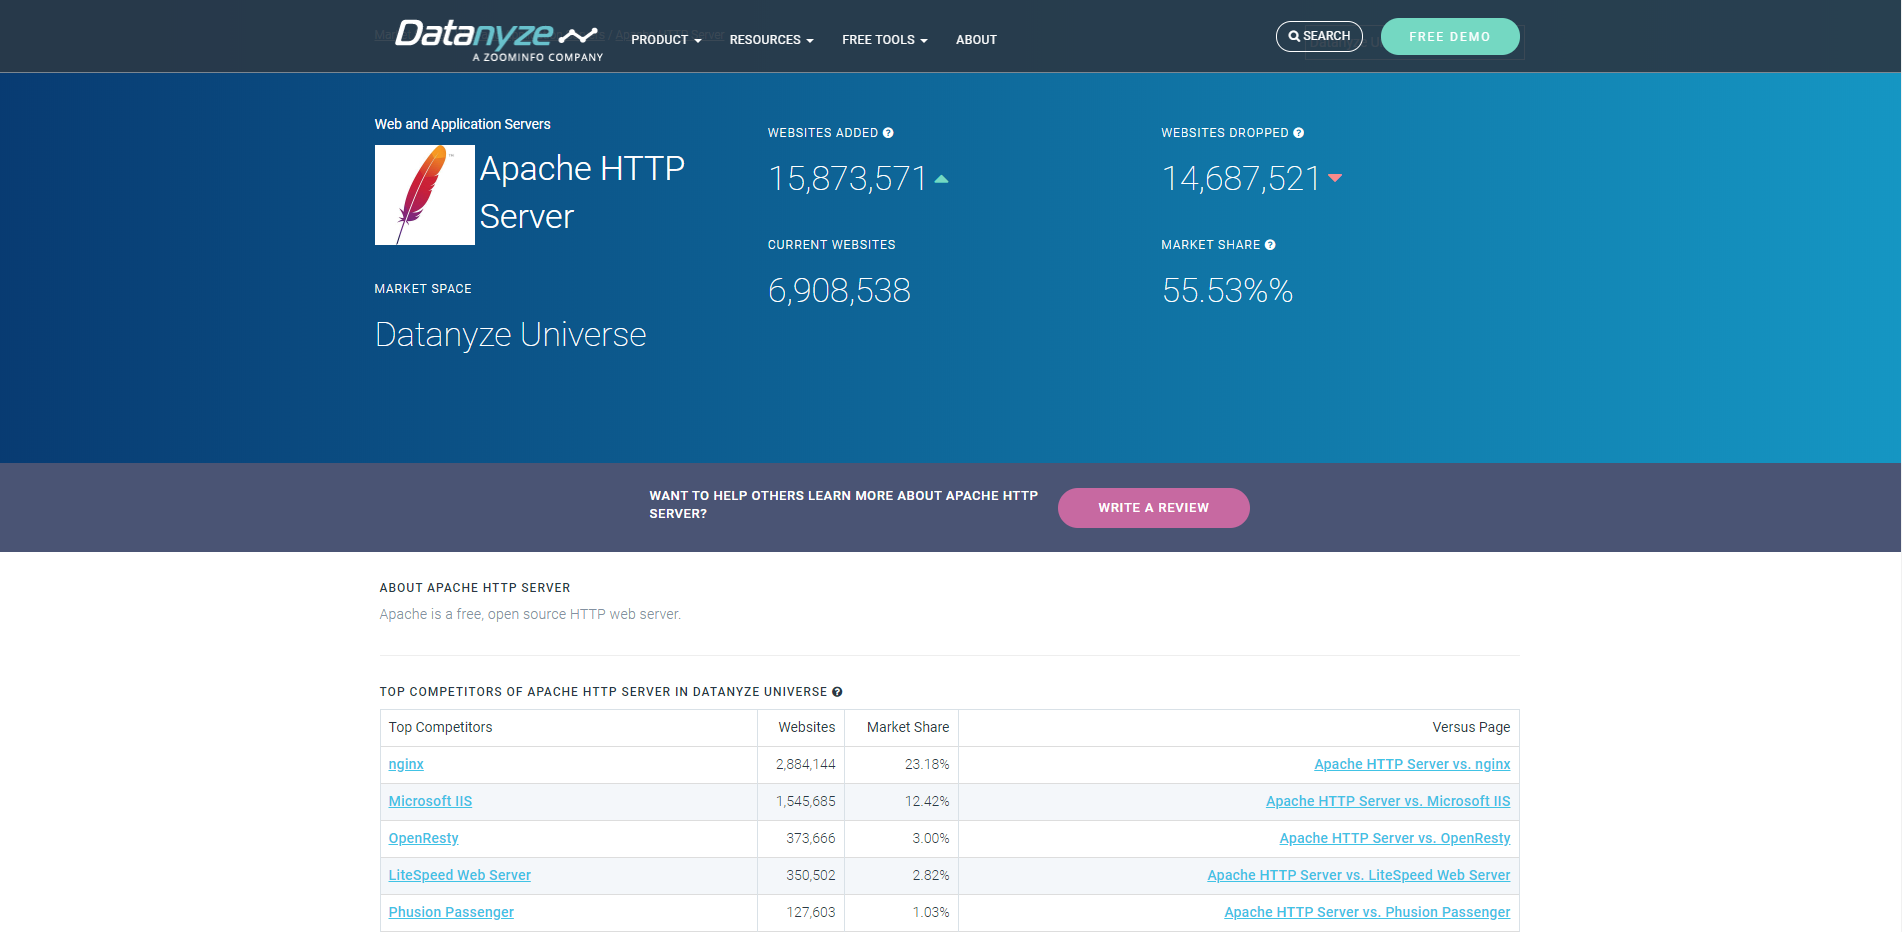
\includegraphics[width=88mm,scale=0.8]{Apdenix/MarketshareApache.PNG}
    \caption{The market share of Apache web servers \cite{Apache}}
    \label{the market share of Apache web servers}
\end{figure}
\subsection*{Learning loop and known IPs} \label{Learning loop and known IP's}

The learning loop described in the MOSCOW shall be fairly basic and the loop will have two primary functions. The first is simply the ability to distinguish malicious IP addresses from the collated data. The secondary function is to identify and flag up potential candidates from the IP collection that could potentially be search engine bots. These requests may have many similarities in architecture. The IP of a bot could have different address patterns, even if sent from the same host, and these bot IPs may change periodically. This would require a larger amount of data input, therefore, it may be easier to have a community driven approach. Due to the potential for abuse such as a hacker adding their IP to the proven bot list, there is a secondary requirement that an overseer approves all the good bots manually.

\subsection*{Database}
For the justification purposes of database type, the different types of database shall be assessed in this section. The first database that has been considered is a 'NoSQL database' namely, MongoDB. MongoDB is a document-oriented database and is currently the most popular 'NoSQL database' at the time of this research. MongoDB makes it easy to access documents by indexing, hence, it provides a fast query response. A great advantage of MongoDB is that it is a horizontally scalable database, and when you have to handle a large amount of data, it is possible to distribute it to several machines (\cite{MongoDB5}). During the development phase there shall only be one user machine. However, during the implementation of the software the server will scale, this is an appropriate feature supporting the justification of MongoDB. MongoDB does not support joins in the way a relational database would; it may slow execution and effect performance (\cite{MongoDBComp}). This disadvantage may have a detrimental effect on the operation of the software, as the data will need to be stored on multiple tables. MongoDB stores key names for each value pair. Also, due to 'no functionality of joins', there is a data redundancy trend. This may result in increasing unnecessary usage of memory and once again is a limitation that may effect the software.

Another alternative database type for the software could be an SQL. An advantage of this database is that by using SQL queries, the user can quickly and efficiently retrieve a large number of records from a database. This would have a positive effect on the processing speed while running the software. In the standard SQL, it is very easy to manage the database system. It does not require a substantial amount of code to manage the database system; this will help to keep the code for the database neat and tidy, and the code required for accessing the database will also be kept similarly trim and ordered. SQL can be used in laptops, PCs, servers and even some mobile phones, which will aid in the development of the software through multiple access vectors (\cite{JavaTPoint}). Microsoft access could be used to develop this software as it is a popular SQL database that can easily be run on a computer with Java integration. If this approach is selected as the database candidate, it would also present a key supporting justification for the utilization of java coding, this will be discussed later in the section on the \nameref{Language} for details.  


\subsection*{API }
A lot of the APIs may be able to provide data to the software, for example, abuse IPs and GOIPs. Free APIs are available from many database hosts that can identify abuse IPs for example (https://www.abuseipdb.com/). This API could be embedded in the software to assist in identifying malicious IPs. An example of an integration technique that is not classified as an API yet still aids in the data provided at the GOIP level is Geolite2. This program helps to locate and pinpoint the coordinates of an incoming IP address hence assists in the identification of malicious IPs. The overall decision to not use APIs was made to keep the data that is collected by the software secure. If the choice was made to allow for APIs it very well could be the case that an attacker may realise that they have been discovered and this may effect the overall analysis of the software.

\subsection*{Language} \label{Language}
Many languages were considered including Python, C, PHP and Java. Java is architecturally neutral and would work particularly well for the project as it can be run on any machine. As many users will be utilizing the finished software on various platforms, the use of Java would be advantageous. The use of C as a language was also considered. The language C runs on many Unix systems on which most servers run, however, in the modern world most website owners do not necessarily have access to the server that their site is hosted on. Another reason for standing against the utilisation of C as a language is that this language may not be appropriate for the development of a user interface that will be required as a vital component of the software. Python was considered as an alternative code for the project, however, the main issue that was discovered with Python was its limitations with database access. If compared to popular technologies like JDBC and ODBC, the Python database access layer is found to be somewhat underdeveloped and primitive. Due to the proposed architecture of the software, Python would not be a suitable language, as fluid database communication is integral to the project. Finally, PHP was considered as a language for the project because the software could be implemented as a web based application. Unfortunately, this approach may have given the attackers access to the data, as it is open sourced. This would defeat the overall objective of the project and the software.  

\subsection*{Data Controller}
The decision was made to limit the influence that the computer has on the mitigation of attacks. Many of the papers mentioned in the literature review applied some kind of machine learning or formulaic protocol to ring-fence potential malicious attacks and mitigate them. In the majority of the papers reviewed, there was a margin of error, or degree of uncertainty with the results due to the methodology in their approach. Due to this, the decision was made to enrol a data assessor to the process in order to filter out the IPs that the software had picked up as potentially malicious. This human approach will allow with 100\% certainty that only malicious IPs will be blocked, reported or otherwise actioned.  \label{Errorcodes}
\chapter{Design and Implementation}
\section{Hypothesis}

The overall question behind the research project discussed in this thesis was to establish whether there was a better way of detecting malicious traffic. In essence, is there a way to identify and flag malicious IP requests with a formula based around the GET request characteristics. However, it would be appropriate to portray the purpose of the research with the following set of hypotheses.

Firstly, it is hypothesised that the process of collecting log files will be an efficient way of collecting data in terms of space and computational resource. It was highlighted in the \citeyear{staniford2002practical} paper by \citeauthor{staniford2002practical} that it is considered completely unfeasible to save all network traffic for any sustained amount of time as there would be too much data to store. Hence, collecting information with variables suitable for study in the condensed format would be invaluable for the performance of the software. This was a hypothesis that was promoted by the issues uncovered during the literature review of \cite{Adi2015} and \cite{Adi2016}. These papers suggested that looking at a large data set may be problematic due to the constraints of processor depletion. It is therefore hypothesised that by only collecting log file data, that is collected by default anyway, will mitigate the workload effects that cause CPU redundancy.

It is predicted that there is sufficient data within the log files in order to diagnose, with a degree of certainty, potentially malicious IP traffic patterns. It could do this by looking at the characteristics of each traffic instance. It can therefore be hypothesised that a formula could be developed as an aide for the identification of potentially malicious IP traffic instances by using the characteristics of each traffic instance and portraying them as variables. It is proposed that the overview of a human moderator could look upon the potential threats and assess their elements. They can then evaluate and take appropriate action, after confirming the status of a malicious IP instance.

It would be logical to postulate that a simple user interface would improve detection accuracy for users. This would be enforced by ensuring that website owners can analyse data in a understandable way. During the literature review there was no study that explored a user interface design specifically related to a detection software. Therefore, it could be argued that there is a definitive need for a user friendly UI, and this should be a critical element in the design architecture. Details and approaches for the intended user interface will be discussed later in the Chapter.

It is hypothesised that using a human moderator in combination with a formulaic detection system, more malicious traffic will be correctly identified and less genuine traffic will be misidentified as malicious traffic. The formula's mandate is to identify potential threats, however, it shall not be used to make the final decision on any IP instance in terms of countered action. Many of the thesis read as part of the literature review used a singular approach of either artificial intelligence or a formulaic diagnostic in order to identify malicious traffic. In most cases these approaches admitted to a degree of uncertainty in their methods of identification. For this reason it has been decided to implement some kind of manual assessment of the incoming data overseen by a human moderator. When implementing a fix for this at the design level, the decision was made to use the access logs which are already collected by default on web-servers as already mentioned earlier in this chapter. The human moderator would then be able to access the full details of the traffic instance and investigate its potential malignancy, hence improving the degree of accuracy of identification.  


\section{Design decisions}

During this section the approach to the software requirements shall be discussed. The requirements are outlined in Chapter 5 and Appendix \ref{Moscow}. Relevant arguments shall be debated in order to comprise best practice for the design of the software, including the justifications for any vital decisions made. The formulation of the design shall in turn be built in order to prove or disprove the hypotheses that have been raised in this chapter. 

When considering a choice of language to use in the software, the following considerations had to be made, after elements of the justifications section were taken into account. The first point that was considered was the primary concern of the software being able to maintain confidentiality and how it may have an impact upon the results of the software. In essence, it is considered imperative to keep the data collected away from the eyes of potential attackers or hackers. For this reason PHP as a language was disregarded, as it would lead to the software being available online. This would make the data potentially available for malicious users to access online. 

It was decided to design the software utilizing an object orientated approach; this approach means that the software can be designed as a series of objects that interact with each other (\cite{OOP}). Using an object oriented approach allows for easier implementation of new data and function as opposed to a procedural approach; this will lead to a more agile methodology when developing the code. Object oriented programming also provides 'data hiding' which in turn, makes the approach as a whole more secure. This was considered a boon due to the fact that this would mean that the data within the program is neatly categorised and sectioned. It is considered beneficial to keep the UI coding separate from the functional code. It is also valid to mention that in object oriented programming, data is more important than function. In the software, data is the most important aspect of the framework and the functionality is secondary. Due to the complex nature of the data driven approach, data could be analysed easily and can be manipulated in many ways to produce logical outputs.

Another language that was considered to be a close contender for the language of choice was C. C would have been an appropriate choice if we were using it on a server due to the fact that C is the base language of servers, as they tend to run unix systems (\cite{ehost}). Due to the complex nature of the program there may have been some issues implementing C as a language. C is a procedural language, therefore, it requires the code to be longer. There are also some inherent issues when using objects to represent data. On the other hand, Java, is built in objects, therefore it is easier to represent complex data structures by using objects. For example, each line in the log file is represented as an object. 

Python was also assessed as a contender for writing the software. Due to the fact that Python is dynamically typed, this would make the task of debugging some errors longer. Java on the other hand is statically typed, it expects the variables to be declared before they can be assigned values; this prohibits running the code if errors are generated. It also means that you are unable to accidentally alter a data file into an incompatible form. The prevention of error and debugging ease of Java were the deciding factors in promoting Java above the other languages. It was concluded that Java was the most appropriate language for the development. 

The database runs as an SQL database, this was chosen above 'no SQL' for the following reasons: The first is that it enables the use of joins, this reduces the data that needs to be stored as some of the data would be replicated. For example, every IP has a type, without join this would need to be a text parameter, hence by using joins we can save the type in a different table and then make reference to them in the IP table. Another reason for utilising SQL is that it is highly compatible across a number of different devices; this would be beneficial to the overall development of the project through ease of access. A third and final reason that SQL was selected is that SQL works hand in hand with Java in terms of compatibility, and as discussed previously, Java was selected as the best candidate for a language choice. 


\section{System Architecture}

This section will look at the design of the software from an architectural point of view, the design of the user interface will be discussed in a later section (\ref{ui}). 

The code is divided into 3 sub-systems; these sub-systems were then made up of relevant files. The first sub-system is the data model; this system is where all the back-end calculations are performed and then passed to one of the other sub-systems. The other two sub-systems are the main user interface and the admin user interface. By designing these three components as separate sub-sections, it enforces a highly cohesive design with low coupling. The systems could be written independently of one another, supporting the agility of the design as a whole. The data model was written first as a basic text output, this aided in design; due to the fact that when it came to the UI, the data that needed to be displayed was already available and calculated. It also meant that pinpointing a formatting error was easier to locate, for example, if the error was in the raw data or the UI. 

After a user selects a file to be read into the software, each line of the data is stored as an object and then each object is placed into an array-list ready for further processing as needed. An array-list is a Java data structure that allows the storage of items. In this particular project, the array-list is used to store a collection of objects, namely the website hits. A hit is defined as one line of data within the log file. The data is stored in an 'object of type' data store'. The data store is then passed between UI's, this results in all UI's being able access the correct data, it also saves passing multiple arrays and maps. This makes it easier to pass the data around the software in a consistent way.

An array-list was chosen as the data structure due to its superior performance (\cite{JavaAL}). Due to the size of the website log-file, in terms of number of entries, the dynamic size of the array-list is more suitable for this project. An array is a fixed size, meaning the only logical way to use an array would be to set the size to a large number and hope no data would be larger (\cite{Array}). After the array-list has been populated it is then sorted into multiple hash-maps so that the data can be easily interrogated, for example: the number of times an IP shows in the data can be saved as a key value pair. 


%Much of the data used to... calculated UI displays is stored as a hash map; this makes it easier to do a lot of basic manipulation of the data. Other types of maps were considered for example a TreeMap however, due to the the fact that a HashMap is generally quicker and the application is not focusing on the order of the IP address, then a HashMap seemed like a better option however, because they all use the map interface, if at a late date a different map would be better, then this could be easily changed. https://www.geeksforgeeks.org/differences-treemap-hashmap-linkedhashmap-java/

Due to the software's heavy reliance on a database architecture when calculating values, it was considered good practice to use a database class to control access to the database. This means that the control of the database is abstracted away from the main code, therefore, it will improve the overall cohesiveness of the software. High cohesion gives the software a better facility for maintenance, while low cohesion results in monolithic classes that are  much more difficult to maintain, and generally reduces re-usability. Due to the complex nature of the design, by having high cohesion, it was easier to insert adaptations during the design implementation.

\section{Overview of the risk factor}
\subsection{Defining Risk} \label{Define Risk}
The judgement of risk related factors is a difficult concept to define and apply mathematical principals in order to construct a logical value. In day to day life risk is a particularly easy thing to identify. It is easy to define whether an event has aspects of high or low risk. However, it is a much more difficult parameter to breakdown and portray in mathematical terms. Furthermore, this software is proposing a technique that focuses on previously unexplored influences. Therefore logic has been applied to define the weights of risk in many cases due to a lack of prior study and research. As discussed in chapter 4, a lot of risks come from the context of the scenario. Therefore, even though this can be mathematically defined, it is important to accept some limitations with the rational presented within this section. The supposition of logic in many cases has not been implemented with supporting research due to a lack of prior investigation. It is even more important to point out that people cannot agree on the definition of a risk. As \citeauthor{fischhoff1984defining} states 'The focal ingredient in all this has been concern over risk. Yet, the meaning of "risk" has always been fraught with confusion and controversy' (\cite{fischhoff1984defining}).

In order to define risk a formula was proposed in order to look at different vectors that became apparent in the log files. Along with this historical data was applied to compose a mathematical assessment of overall risk rating. It is believed with these two key principals for defining risk, the assessment of incoming traffic can be asserted in terms of its potential for maliciousness.

The body of the risk factor was made up of two distinct partitions. The breakdown of this value is made up from the first partition; 90\% coming from the formula itself. The formula itself will be discussed in section \ref{The Formula}. The second partition is comprised from two smaller sub-partitions and makes up the remaining 10\%; this is comprised from historical data gathered within the database. The two sub-partitions making up the remaining 10\%  have separate weights values. The first is data collected from the last 30 days and given a 75\% weight, the second is data collected from all time and given a weight of 25\%.

The use of the historical data is to try and give the system some idea of context, as it helps the system see if an IP has shown up and been reported in another log file. A paper by \citeauthor{reiss2007efficient} looks at the ever evolving methodology in utilising streamed data for research. \citeauthor{reiss2007efficient} states that: "While current reasoning approaches are designed to work on mainly static data, the Web is, on the other hand, extremely dynamic: information is frequently changed and updated, and new data is continuously generated from a huge number of sources, often at high rate. In other words, fresh information is constantly made available in the form of streams of new data and updates." (\cite{reiss2007efficient}) As assessing streamed data is a relatively new concept, it would be reasonable to assume that more recent data, is more relevant data. Therefore a heavier weighting is given to the last 30 days as this is to try and assess if the IP is currently or actively attacking other websites. In addition to this, IPs sometimes change, this was why after 30 days a lesser weighting is given to the IP. It would be appropriate that this factor still forms part of the calculation. This is due to the fact that an IP may be used in rotation therefore, it may be quiet for a while and then begin attacking websites again. 

Users have to manually report suspicious IP addresses; this was a design decision that was hard to make due to the opposing views of the literature. There is an argument that the IPs should be automatically reported to the system and this would have given the system more data. It all comes back to context, in which case a human is better placed to judge, and do so more accurately than any mathematical generalisation could. A human could appraise a variety of factors that a computer could not compensate for. An example could be presented where a user's personal IP would show up more frequently than any other traffic instance; this would potentially lead to a high risk related tag. This reinforces the case that there was the chance that non malicious IPs could be flagged and reported to the system. 

As previously discussed, 90\% of the weighting is derived from the data contained in the log files; this may be regarded as a particularly heavy weighting. The rational behind this decision was due to the IP activity on a website being assessed independently of other websites. The high weighting of the log file means that an IP, even if not known to the database, can still achieve a very high risk factor, providing user feedback about their log file. In the next section, this thesis will analyse the inner-workings of the formula.
%.Why we use historical data
%.the fact that users have to report the data
%.Why some some elements weight more than others.

%end with intro to formullaz
\section{The Formula} \label{The Formula}

As was mentioned previously in this chapter, the formula itself is the key factor in defining risk. It is believed that it shall go a long way in diagnosticating the malignancy of malicious IP traffic, while deescalating false alerts with similar architecture.

The formula is broken down into five distinct categories of information, these five variables were chosen as they each look at a different architectural aspects of a traffic instance. It is believed that a malicious IP instance can be detected and identified by looking at the values of these attributes. The code for the formula can be seen in appendix \ref{code}.

\subsection{Bots}

It is well known that bots are used by numerous online companies in order to index and categorise various web-pages. Although some of these instances of traffic can at first sight appear to be malicious, due to their architecture, they are in fact a legitimate form of web traffic. For this reason a process is required within the formula to disclude known bots from any further processing within the formula and disregard them at the identification process. This process should preferably be carried out at an early stage within the program. For this reason it has been decided to set this risk factor to zero for known bots, as they pose no risk to the website.

The data for bots is gathered from other websites and deposited in a database where an admin can sort them. The formula will access this database to search for known bots. According to \citeauthor{Bots} 17.5\% of web traffic was determined to be legitimate bot traffic, for example: Google crawlers. These bots are vital for the maintenance and navigation of the internet, hence the importance of the software to disclude these IP addresses from potential barring. It is suggested that 20.4\% of all web traffic in 2018 was considered to be malicious (\cite{Bots}), most of which was automated in a bot like format.

Due to the fact that fake Google bots or fake search engine bots exist online (\cite{algiryage2018distinguishing}), this first check could be altered in the future to look at whether a bot instance is legitimate. The decision was made not to implement this as part of the formula during this research. The reason for this decision will be discussed during the final conclusions of the research.

 
\subsection{Number of Requests}
The literature would indicate that the more requests a website receives from a single IP, the greater the likelihood that the source IP is malicious. After consideration, it was concluded that an IP occurrence may appear in the log files a large number of times: this may result in an over-inflation of the risk factor. In order to mitigate the potential for this event the decision was made to implement a natural logarithm in order to normalise the data into a more collective state. This, in turn, will help to generate a risk factor that has less chance of procuring a large anomalous value, hence breaking the formula.

An alternative measurement could be formulated from the log file data. This would be done using the time between each successive instance of the same IP address. If the time between each successive instance of the same IP traffic is very small, these types of attack are better mitigated in real time. Cloudflare states that 'ability to implement page rules and populate those changes across the entire network is a critical feature in keeping a site online during an attack'. There is a possible situation that could occur, where web traffic from an IP may come at a staggered rate, however, this may also have the same affect, and the same potential for malignancy. 

After careful consideration it was decided that it would be better to test more attacks by looking at the average time between IP instances; this was generated using the following formula: \[\lnb{\dfrac{Occurrences of IP }{43800 \times No. of log files}}\] It must be noted that the minimum value of this is 0.1 in order to prevent errors in the calculation. 

It would be appropriate to include an explanation of some values within this formula. The figure 43800 is the average number of minutes in one month, based upon 30.4 days being the average number of days within a month. The number of log files is a dynamic value based on the number of files that have been uploaded to the software. This allows multiple months worth of data to be analysed in one sitting.

\subsection{Response}


The response of the server is a good indicator of the legitimacy of a request, the server assigns a http code to the response. The decision was made to break down each request/response and apply an applicable risk level for each response code. The justifications for the applicable risk factors shall be discussed within this subsection. It should be noted that none of the literature reviews used this as an indicator for attack identification. As this is a path finding approach, the application of a risk factor for this element may be more likely to be adjusted through critical review after testing (\cite{ErrorCodes}).

A \textbf{400} error implies that the IP traffic instance made a BAD REQUEST. This would suggest that the user did not come to the site on a natural path from browsing. It would suggest that an error in logic was established during the request. On some web-servers a 400 error message can be broken down into more detail to pinpoint the architectural issue within the request. It should be noted however that the web-servers used for testing with this software do not use  IIS 7.0, IIS 7.5, or IIS 8.0, and as such will not break down full details of these 400 errors.

An invalid timeout response could be indicative of a situation where the GET request packet is invalid or has poor flagging standards. This could be a sign of a low rate bandwidth attack, hence it would be appropriate to apply a risk factor association for the greater 400 response error. 

An invalid destination header might suggest an incorrect http pathing request was inputted and may be indicative of a BOT attempting to formulate potential page targeting unsuccessfully. It may also indicate a handcrafted packet that has been constructed incorrectly or synthetically. As discussed in the literature review signs of a synthetic packet are highly indicative of a malicious request.

Due to the varied vectors that can produce a 400 request and the commonality of this error, it would be fair to apply a risk factor that does not overly penalise the event. After consideration, a lower weight was applied to this error response with the ideology that it may stack after repeated instances of the same error.

A \textbf{401} error would indicate that the user is not authenticated to view the web-page. This could be due to an error in the server settings, which may lead to further unauthorised probes to evaluate weaknesses in the server configuration. This could also be an error raised from the occurrence of too many consecutive requests from the same IP or that the maximum number of allowed requests has been met. This would indicate that perhaps a server owner has set a limit on the amount of IP requests from the same source. There may however, be legitimate reasons for a large number of requests from the same IP within a set time frame. A 401 may also occur if the website runs an API service, the API may generate a 401 error due to invalid credentials. These error messages should be given a suitably high risk factor rating as they are attempts to access forbidden pages or instances of denial. 

A \textbf{403} error is similar to a 401 in that a visitor has passed the authentication stage for reaching a page, however, for some reason they have failed to be permitted access to the page; this could be due to a read, write or execute violation. It could be an error generated from the denial of an IP even if an IP has been rejected due to historical data filtering, this would still generate a 403 error message. Therefore, this would suggest that this specific instance of traffic is most probably an attack, and also most probably automated. This would be fortified by the conclusion that, if a genuine visitor received a 403 message, they would eventually stop sending requests. Alternatively, an automated bot attacker would send a string of requests and continue to receive 403 messages. After consideration it was decided to give this error message a fairly high risk related flag.


A \textbf{404} error is an indicator that the page requested has not been found and is perhaps the most common error response encountered during response protocol. This potentially could mean that a visitor may be searching for a page that does not exist. Although this could be accidental or due to a change in directory navigation. If the error is repeated then this could be a sign of malicious activity. Due to the potential of an accidental or genuine 404 error, this was given a nominal risk factor for association.

A \textbf{429} error flags a scenario where a visitor has made too many requests within a set period of time; this could be indicative of a flood attack or a Denial of service attack. These appear to have a distinct overlapping with some of the criteria for a 401 error and therefore a similar weighting methodology should be applied. 


A \textbf{500} error tends to indicate where the IP is requesting data from. This could be an internal error such as the server is too busy. This may in fact be an indication that the server is under attack from a DoS attack, but does not suggest that this particular IP instance is the culprit. On the other hand, this could also be due to a rewriting or data storage error on the target servers. It could be argued that this is a negligible risk factor however, a repeating IP receiving this response could accumulate a fairly high risk score. This visiting IP would begin to appear as the main culprit of a DNS flood attack through multiplication of this smaller risk factor.

A \textbf{200} response suggests that the visitor request has been successful; this is a potential indicator that a request is legitimate, however, in the case of some discreetly synthesised attack packets, this is not always the case. For this reason a small risk reduction should be applied in order to mitigate risk factors from other variables. The response risk is a signed integer, therefore when you make a large number of requests that return a 200 status the risk factor will be significantly reduced.



\subsection{Pages accessed}

The pages accessed from each visitor could be indicative of a malicious IP traffic status, hence some elements of risk should be appropriately applied. Firstly, if an IP is attempting to request access to WP-admin, which is the standard administrative area of Wordpress websites, it would be appropriate to apply a moderate risk rating. It is common for attackers to attempt brute force attacks at the "WP-admin"; this is typically an attempt to unlock associated admin passwords by flood attempting a guess system in order to bypass security (\cite{Brute}). The attacker, which is normally a bot, will try as many username and password combinations as possible until they find the right one; this makes accounts with weaker password combinations particularly vulnerable, for example 'password123'. It should be noted that there may be genuine reasons that users may need to log into WP-admin. For example, a blogging website may have multiple bloggers, hence the reason numerous individuals would require access to the WP-admin page.

If an IP searches for a page containing the word 'login', it would be appropriate to apply a nominal risk factor. This could, however, be a genuine request, the majority of authentic visitors would tend to navigate to the page by a procedural method. It should be noted that if there is no page containing the word login, they would get a higher risk rating cumulatively, due to receiving subsequent 404 errors, hence, distinguishing a malicious trend in the activity of the IP. The inverse is true if there is a login page, then a 200 response status would be applied to the communique, reducing the risk factor slightly.

Although the formula has variables that appear at first to be separate and independent, by combining the risk related data enables the building of a 'larger picture' of the trends associated with a visiting IP.  An example of this would be the status and the requested URL. Through correlating variables, malicious access attempts are highlighted and less aggressive traffic is mitigated accordingly.

The response size should be taken into consideration as an element of potential malignancy. If a request generates a server response with a size of zero, this may signify that the connection was closed before a response was returned. An event such as this could be indicative of a bot attack, or perhaps a GET request containing inappropriate flags.

\subsection{Country}

After consideration of data made available online, it appears that the country of origin for IP traffic can potentially infer a greater risk. After intensive research during the writing of this thesis, it was discovered that the USA was the origin of 45\% of all malicious traffic (\cite{Webattacks}). It should also be noted that the USA has the third highest population of active internet users in the world. Interestingly, this factor does not diminish the phenomenally high percentage of malicious traffic coming from that country. It therefore would be negligent to dismiss a country risk factor from the origin of IPs. It should be noted that some countries, such as China, have a particularly prohibitive fire-walling for internet access which is enforced through governmental regulations (\cite{China}). The possibility of forcing malicious traffic from countries such as China through a VPN or proxy, in which case the initial country would be disguised from the software is a limitation that can not be underestimated. It is important to note that although the software has the ability to detect the country of origin for the IP source location, it does not have the ability to assess the target websites location. This illustrates how important 'context' is, as for example, a letting agency in the UK would expect a higher rate of UK IP traffic. This highlights the importance of a human decision maker within the detection methodology in order to access the risk related factor in terms of the context of the event (\cite{cranor2008framework}). Due to the increasing ability for users to mask their location online it may be unfair to allocate a high risk factor for this element. Instead it was more appropriate to apply minimal risk factor in order to assess its effects upon the monitoring of potential threats.

To illustrate the risk factor for country of IP source it was decided to rate each country in terms of risk between 1 and 100. These were formulated using the data supplied at the time of research from (\cite{Webattacks}). A percentile approach was used to illustrate risk scoring based on the number of attacks that had originated for the country source from the statistics from this website. There is a UI built into the admin section that will allow an administrator to update the country risk. The logic that is mentioned above is enforced.

\subsection{Conclusion}

After consideration of the numerous risk associated variables, the following risk weightings are proposed and have been documented in appendix \ref{Weights}. As has been shown in section \ref{Define Risk} there are inherent difficulties in defining risk using a mathematical approach, however, by utilising the information documented in the section above it is imagined that the following mathematical methodology can be used to define the risk of web traffic instances. 

\[risk = (orrcancesOfipLog \times 0.6) + ((requestRisk+responseRisk) \times 0.3) + (countryRisk \times  0.1) \]

It is believed that this formula would in part go some way to replicate the intuitive process that a human moderator would go to in order to diagnosticate malicious traffic. After running data through the formula, the outcome shall be a value between 1 and 100, the final integer is the value shown to the user in order to indicate overall risk. It is important to correctly weigh each variable with the appropriate \%. After careful analysis of the threat vectors it was decided to give the largest weights to the occurrences of IP. The decision was made to do this, as the vast majority of attacks share a correlated feature of large numbers of successive visits to the same site from the same IP. 

The request and response is the second most important factor in the formula; this is the accumulation of the response codes and the request is the page they are attempting to access. These two factors are combined equally to make up the 30\% portion of the overall formula. The decision to apply this weight was due to the multitude of different associated code risk factors. An accumulation of internal response events could have too much impact upon the overall outcome of the formula if the weight was set beyond 30\%. These variables are calculated independently as in future these may require separate weights.

As discussed during this chapter, the country of origin is a particularly difficult weight to define. It has not been used as a key indicator of risk factor in prior methodology, hence, it is a relatively experimental risk flag. It must also be noted that due to the increasing use of VPN activity online, it is becoming more and more unlikely to know for certain the true country of origin for any IP source (\cite{GoGlobe}). Hence the risk factor is at this experimental stage, particularly ineffectual on the outcome of the overall formula.


\section{UI design} \label{ui}

As previously discussed in Chapter \ref{Human factors} it was clear that the user interface is a vital component in the process of accurate identification of malicious traffic. It was illustrated by prior research that novice users with little or no knowledge of Cyber security have a tough time identifying malicious activity. However, it is possible for them to do so given the correct information in a clear and self explanatory format. Given the conclusions from research that observed novice users when approaching the detection of threats, it was good practice to apply the utilisation of Nielson's principals. Consulting these principals aided in the construction of a user interface that promotes understanding and ease of functionality.

A minimalistic design was chosen for the creation of the UI. One of Nielson's 10 heuristics for user interface design warned that 'Dialogues should not contain information which is irrelevant or rarely needed.' For this reason a UI based around functionality over aesthetics was chosen as a fundamental for design. The UI is particularly basic, however, it displays the relevant data to the user and is highly functional. The overall log file data is broken down into three distinct categories with clear and self explanatory headers supporting the usability for non expert users.

To aid the user experience, when a window is closed, the software goes back to the previous window. Each of the two main UI sections are centred around a main interface. The website owner interface is centred around the data from their log-files and when they click on one, more detailed data is shown, this includes the calculated risk factor with a coloured bar: coloured green below 25\%, yellow between 26-50\%, orange between 51-75\% and red 76\% and above; this gives a very quick visual indication of the risk associated with the IP being looked at. 

Within the UI the decision was made to use clear and simple English and avoid the use of codes and complex terminology. Nielson suggests that a designed system should speak the 'users' language', with words, phrases and concepts familiar to the user, rather than system-oriented terms, that follow real-world conventions, making information appear in a natural and logical order. This approach is supportive to novice users and aids in their understanding of the software.

The user interface was constructed with data aligned to clear columns and lines in order to keep the format neat and tidy, and draw the users eye to appropriate data fields. \citeauthor{cranor2008framework} stated that the implementation of system features that are intuitive, and simple to use will help to support a novice to engage with them (\cite{cranor2008framework}).

The user interface that shows the risk of an IP is made up of two separate tabs. The first tab shows a high level summary of the IP including: Times visited, total data sent, country code, times reported, reports in the last 30 days and agent or bot status. These data fields were chosen as they give the user a very quick and easy way to see if an IP is malicious. The second tab provides a more in-depth view of the raw log file data, it was important to include this for more advanced users who may wish to interact with the raw data. Even though the data is presented in the same way as the log file, it could be argued that it is easier to understand as it is only showing data from an IP rather than all IP addresses. IT is important to note that the risk factor is displayed on both screens, so the user is not disadvantaged for using either tab.

Nielson stated that Flexibility and efficiency of use is an important factor when designing a UI. Adhering to this principal would support the usability of both basic and advanced features. This is an imperative methodology of design which allows for novice users to use the basic fundamentals of a UI, while allowing experts to learn and excel. While designing the UI, the decision was made to add an internal tab for full details of an incoming IP. This, may be overwhelming for a novice user, however, an expert user could derive much more information regarding the instance of incoming traffic from the use of this feature. Even though this is still raw log file data, it could be argued that it is easier to interpret than the raw log file, as it only pertains to a single IP.


The implementation of Error messages has been applied to the user interface. These messages are generic to maintain the integrity of the software. They are simple to read and understand for even a novice user and help users recognize, diagnose, and recover from errors within the software. This is in line with Nielsons principal for self explanatory Error message presentation. Nielson reiterates the importance of a user interface to support Error prevention. Even better than good error messages is a careful design which prevents a problem from occurring in the first place. The user interface has adhered to this principal as when an IP has been previously listed as a bot, the software has been built to prevent the user from reporting this as a bot a second time.


\chapter{Testing}

\section{Test Plan}

Although the usability of the software is important, as outlined in section \ref{UI Theory}. Due to the scale of testing that would be needed, and recruitment issues outlined in \cite{ben2015effects}, it was decided that user testing would not be carried out. This was down to an an amalgamation of constraints including time and resources. The testing was also due to take place during the first quarter of 2020, however due to the Covid-19 outbreak it was not possible for this testing to take place. As a result the focus was directed towards better "proving" that the formula was able to identify and classify attack traffic. 


As Nielson's 10 rules for design were consulted during the design stage of the user interface, this will be a good offset to critically evaluate the state of the User Interface (UI). Although this may not fully test the hypothesis 'a simple user interface would improve detection accuracy for all users'; this will highlight whether or not the UI has been created with clarity and simplicity in mind. It would be appropriate to suggest that this hypothesis could be further tested in the future through intensive user trials. In order to conduct these trials, intensive user interface testing would involve the recruiting of two groups of users, both 'experienced' and 'novice'. It is proposed that each of these groups would be comprised of a fairly large number. At this time, due to the lack of resources, incentives, and legal issues that arose through the Viral outbreak this would be impossible.

In order to test the hypothesis, the following methodology shall be used to implement a testing approach. A collection of three log files shall be randomly selected from different websites held by a specific server provider. The author of this thesis has managed to gain access to this data in order to test the software at this developmental stage. The log files will contain all IP GET requests that have made contact with these websites within a period of one month. Each of these individual IP traffic instances shall be run through the formula, before being displayed in a graph. The plan of action is to use the log file data to indicate any potential malicious traffic. Further to this, it is the intention to critically assess some of the high ranking IP instances individually, in order to analyse the architecture of each traffic instance. It is hoped that by doing this the hypothesis that 'there is sufficient data within the log files in order to diagnose with a degree of certainty, potentially malicious IP traffic patterns' shall be consolidated with an answer. 

An alternative method of testing was considered, this was to take 4 random IP instances and run them through the formula for critical evaluation. However, this methodology was set aside as choosing 4 random IPs may have provided trends or flags with very similar characteristics. If the 4 IP instances were chosen by picking IPs with different trends or flags, this may have lead to criticism of bias and may have invalidated the research. By assessing a larger data pool it is easier to highlight any instances of outlying data and whether or not the system can classify malicious traffic.

The way in which the hypothesis is tested by collecting log files, will be an efficient way of collecting data in terms of space and computational resource; this shall be done by assessing whether it was possible to detect any malicious traffic using the log file data. If this was possible, then it may be concluded that the spartan amount of data collected would in turn have a dramatic effect on reducing computational resources. It should also be noted that to do alternate full testing regarding CPU depletion, would involve monitoring all CPU processing on the server of a website for one month. This is both impractical and intrusive. It should also be noted that a website tends to run email and other services, thus, it would be problematic to identify the depletion that accounts for the log file data collection.

In order to test the hypothesis that 'by using a human moderator in combination with a formulaic detection system, more malicious traffic will be correctly identified and less genuine traffic will be misidentified as malicious traffic' the following proposal is made. A test could be performed that finds a semi anomalous reading in the log files with malicious 'trends'. If this particular instance is flagged by the software as being a high risk candidate, but is not a malicious entity the hypothesis has been proven. This is simply due to the fact that the system would have assessed this as a malicious threat, however, after being analysed by a human moderator, the appraisal of context lead to it being descaled as a false alert. It is, therefore believed that this would inherently prove a 'human in the loop' has enhanced accuracy of detection. 

In order to test the ability of the system to detect bots, an IP from the log files that exhibited bot like behaviour was selected and tagged with TEST. In theory this should be picked up by the software in the ANGENT or BOT field within the summary tab inside the UI. This was implemented in order to support the MOSCOW element, proposing that the software MUST 'be able to add or remove a known IP address' for services like google and Bing bots.

A small modification was made to the program in order to enable it to look through all of the IP addresses and work out the risk factor, as well as the number of occurrences. The software then logs this data into a CSV file, where it was displayed in a graphical form, the data can then be interrogated. The results will be discussed in the next section.
\section{Evaluating the Formula}
In this section, the formula, that was discussed in chapter 6, shall be evaluated in order to assess its ability to detect malicious trends in traffic. This thesis shall then go on to evaluate the UI in terms of its functionality, by doing so, the hypotheses raised in the prior chapter shall be evaluated.

Three websites were assessed over a one month period and log file data was collected from each site throughout this period. The data captured from the website logs was taken in late January and early February 2020. It should be noted that two variables were chosen in order to display the data and results in a graphical summary. These represent the risk rating versus the occurrences of the IP. The risk rating is an obvious choice for a variable due to the fact that it is the key focus of the software and the proving factor for the majority of the hypothesis. The occurrences were chosen as the second variable due to the fact that they were the aspect that were given the highest weight rating in terms of risk. If the researcher were to look at the requests and responses, they would need to log every occurrence of each response code, which would be difficult to display in the form of a graph.



After looking at the graphical display of data, as it can be seen in Appendix 
\ref{Graph data}, it was clear that a trend exists between extreme levels of occurrences and a higher risk rating. Six out of nine IP addresses with occurrence counts of over 1000, fall within the highest 0.3\% of risk ratings. It should be noted that a huge number of IP addresses seem to fall into the categorisation of low risk rating. 99.45\% of readings fall into the banding of a risk rating of less than 10. For the purposes of testing, in order to analyse the formula in detail, the 10\% from the database that would normally contribute to the score was ignored, therefore if an IP got 100\% in testing then this would equate to 90\% overall.

In order to evaluate the elements of these results it was decided to take some of the IP instances with the highest risk related factors and attempt to diagnose them as malicious or genuine. The decision was also made to look at some of the more anomalous readings, particularly those that fall far outside of the 'trend-line'. These values tend to be those with particularly high occurrence ratings and yet with low risk factor readings, or those with large risk factor ratings and particularly low occurrence ratings. The architecture of these traffic occurrences shall be evaluated individually in order to make conclusions regarding whether or not they display any signs of being a malicious entity.

\subsection{Detailed look at IPs }
In order to further assess the capabilities of the formula. Seven IPs shall now be cross referenced with the data held on abuseipdb. As discussed, these IP's were those displaying the highest risk rating score, and also those falling far from the 'trend-line' on the data set. It is anticipated that this will show the ability of the formula in detecting true attacks.

\subsection*{194.61.24.46}

This IP address originated from the Netherlands. After corresponding with the abuseipdb it was found that this IP has been reported a staggering 1104 times due to malicious trending visits to other websites. After looking deeper into the raw data, it was clear to see that the chains of 403 and 404 responses were patterned in a systematic repeating cycle; thus it is is fair to conclude that this is a malicious entity with bot like features. The software was able to flag this and gave the IP a risk related scoring of 100/100.  

\subsection*{209.124.66.6}

This IP address originated from the UK, this would be a 'best fit' source location to signify a level of inherent trust, due to the UK based websites used in testing. However, when consulting with abuseipdb it becomes apparent that this IP address has been reported for malicious activity 14 times. The formula inferred a risk related rating of 100/100 for this IP source, and the IP was the source of 9134 requests from one particular website within the test window. The responses allocated to the IP GET requests across the test window were made up of chains of 301 and 404 errors. While a 301 response, indicating a redirection for a URL has not been given a risk related factor, in this instance, the continued appearance of these responses are particularly indicative of a potential threat. Along with the 301 responses, a huge string of repeated and systematic 404 errors were returned to the IP source. Altogether it is clear that this IP is the source of malicious traffic, and the formula was correct in applying a maximum risk related flag.

\subsection*{86.175.235.192}

This IP originated in the UK, and it would be appropriate to discuss the features of the IP address and why it may not be malicious. This IP was allocated a risk rating of 100/100, however it is believed that this was a false alert. Firstly this IP has never been reported or raised as a candidate for malicious activity on abuseipdb. The request pattern of the IP address appears to be random in nature, therefore, this does not indicate a bot, as this would be in a systematic pattern. In addition to this, there are a number of 200 response codes, therefore, indicating that some of the requests are legitimate and only some of them are not. An explanation of the pattern may be that the website to which this data belongs was under development; this would generate errors during the testing period. It may therefore be reasonable to predict that this is administration activity. If this is the case it raises a concern regarding the possibility of a false alert being generated by administrators during the building and testing phases of website design. If the rationale that has been adopted to explain this anomaly is correct, it raises the importance of having a human moderator in the detection methodology. Any experienced user would be able to identify their own IP address and de-escalate this false flag.

\subsection*{35.187.118.51}

This IP had the highest number of occurrences within the testing period. Its risk factor hit the maximum score of 100/100. After further study of the data set, it appeared that this IP had made contact with a single website an astonishing 800 times per day, during the period of data collection. After cross referencing with abuseipdb it was found that this IP had previously been reported as a source of malicious activity. The source of the IP was identified as the USA, therefore has a risk related country of origin factor. The raw data within the log files shows a huge string of repeated 403 response codes. This is indicative of malicious activity due to repeated, bot like, attempts to access forbidden pages. It is therefore concluded that this is almost certainly a malicious IP due to the repetition of unauthorised attempts. It is clear that the software was correct in its assessment that this was a high risk candidate.
\subsection{Anomalies in the Data}
\subsection*{192.173.3.114} 

This IP was randomly chosen to be marked as a BOT with the name of "Test"; this was done in order to check whether or not this feature of the software to detect known bots worked efficiently. This IP was marked with a risk factor of 0/100 which supports the conclusion that the software has the ability to detect functional benign bots. When looking on AbuseIPDB, it would appear that this IP address belongs to the University of Northumbria. Therefore, in response to the purpose of testing, it was able to show the ability of the software to detect bots that are known and flagged as such on the database.

\subsection*{108.162.220.175}

This IP originated from the USA. It was allocated a risk score of 6.46/100 through the formula, yet had a particularly large number of occurrences during the data capture. After exploring the raw data it appears that this is an unflagged bot for a service that monitors the 'up-times' of websites. The GET requests generated a multitude of 200 responses which as discussed in prior chapters help to diminish risk related scoring. If flagged properly as a 'good bot', this IP would have been given a risk score of zero. The instance clearly illustrates that particularly high numbers of IP requests within a time frame do not always lead to a high risk related flag. 'Good' or 'genuine' behaviour is credited through the software and leads to a low risk rating despite the weight of the request instances. The software concluded that this IP was a low risk visitor.

\subsection*{63.143.42.250}

This particular IP originated in the USA. At the time of testing the database held on Abuseipdb it was found to have been reported 14 times previously for malicious trending activity. This IP made contact with one particular website during the testing capture 1173 times. After opening the raw Data, it became apparent that this source was a another genuine bot for an 'up-time' website. After looking deeper into the reports on the Abuseipdb website it would appear that the reports were automatically generated by the sites via automated code parameters. Due to the chains of 200 responses a suitably low risk factor rating was issued by the software for this IP, scoring 5/100. This particular log file was instrumental in showcasing the ability of the software to down rate a previously unlisted 'good bot'. Once again, this scenario also shows the usefulness of a human moderator within the detection methodology. The ability of a moderator to use context and rationale within Abuseipdb helped to assess the benign nature of this bot-like activity.

\subsection{Summary}

It is clear from the evaluation of the formula that it is working correctly. Although some false alerts were generated, these cases were identified in essence by the researcher. This action simulates the comparable actions that a potential human moderator could take as the overall system for identification of threats had intended.
%MUST CHECK IF WE NOTED THAT WE HAVE SPOKEN ABOUT THE  10% PART OF THE FORMULA BEING TREAT AS 10/10 FOR THREAT LEVEL DURING TESTING.
\section{UI testing}

Although the UI is not a major part of the project, it is still important to check that the UI incorporates the core functionality required for the system. Therefore, the UI was tested as the software was being built. All components of the the UI were functional as they were implemented, however, when looking back over the software it was found that there were some errors in the spelling of words. Some text fields also needed to be reworded in order to aid the user experience. Formal user testing was not implemented due to concerns over participation and candidate correspondence during Covid-19. It was believed the only way to test the UI properly was to enroll both expert and non expert users to evaluate the UI efficiently. The potential for future testing of the UI shall be discussed during the conclusions section. As mentioned in prior chapters the UI was built in accordance with Nielson's principles and criticisms of this shall also be debated in the conclusion of this work. 

During the agile build methodology, small changes to the UI were made in order to improve the user experience. The changes that were implemented during the design and testing phase shall be laid out in this section in order to present the efforts that were made to encourage smooth human-computer interaction.

It was noted that whilst the button that is required to read the file is present, it does not clearly highlight how to display the data. It would have been useful to make this button clearer in some way, however, due to the time constraints of this project this would require extensive reworking of the program which the aforementioned time constraints did not allow. By adding the words \textit{start here} to the button; this highlighted the button's presence and provided clear instructions on how to start the process.

Many of the Text fields in the UI were altered during the implementation of testing as it was believed that the wording may have been counter intuitive to non expert users. The header 'page' was changed to 'page accessed' to reflect a more self explanatory notation for non expert users. The second search box was removed as it was deemed to be superfluous and may have lead to confusion for users. The changes described in this section can be found in Appendix I.
\section{Data not included in the Formula}

The formula as it stands is able to detect attacks with a fairly high degree of accuracy, however, during the testing it became apparent that some data was not taken into account. It should be mentioned that for the purposes of this formula, the difference in HTTP1 and HTTP2, in terms of security, has not been assessed and appraised with a relevant risk rating. This risk related element could have been added to indicate whether the connection was secure mainly due to the fact that HTTP2 only works on a secure connection. This could have been used as an indicator of how guarded the request was, HTTP1 can operate on an unsecured connection, therefore the data that is transmitted is unencrypted and less secure. It could be argued that a greater risk factor could have been given to HTTP2. \cite{tripathi2018slow} pointed out that HTTP2 had more threat vectors than HTTP1. Due to the evolution and the work in progress state of HTTP2, it was decided that it was a better idea to leave the risk related appraisal of these protocols out of the formula. This was mainly due to the fact that there was no way to guarantee that the HTTP2 protocol remained un-patched and unaltered throughout the timeline of this research.

Due to the time constraints of this project, certain factors that should have been considered were left out. Firstly, the timezone from which the log files originated, and secondly the timezone from which the IP hailed. This would allow the software to calculate the correct time of day that traffic appeared on the website. This was largely down to the fact that to accurately use this data, the local time of the IP address would have needed to be calculated, then a further risk factor plan would be required. This would be a difficult factor to apply risk to, due to the 24 hour nature of the internet.

It would be worthwhile mentioning that certain return codes were not allocated risk ratings as part of the request/response factor within the formula. These in general are not considered to be risk related returns and are mainly indicative of page redirects and paid content response, hence, the omission of these factors from the formula was considered of negligible effect.

\chapter{Conclusions}
\section{Evaluated Hypotheses}

In order to make a complete analysis of the formula and software it would be good practise to review the three main hypotheses.  

Firstly, it was hypothesised that the process of collecting log files will be an efficient way of collecting data in terms of space and computational resource. It is believed that this particular hypothesis was answered simply by building a system that uses only log file data. This data is automatically collected by websites and does not generate any additional computational activity. The data is relatively easy to store and takes up very little space. This hypothesis has been addressed to satisfy the criteria, as outlined in the requirements specification.

The second hypothesis is the prediction that there is sufficient data within the log files to diagnose with a degree of certainty, potentially malicious IP traffic patterns by looking at the characteristics of each instance. This hypothesis was satisfied, as the evaluation of IP addresses that had been flagged by the formula as high risk, were concluded to be malicious by a human analyst in Chapter 7.  

It was finally hypothesised that by by using a human moderator in combination with a formulaic detection system, that more malicious traffic will be correctly identified and less genuine traffic will be misidentified. During the evaluation of high risk scoring IP instances in Chapter 7, several falsely flagged entities were raised as malicious by the formula. The analyst was able to look into the log files and in each case apply logic to assess each instance on its own merits, then conclude that these high risk candidates were not malicious. This in turn supports the hypothesis, as without the human moderator, high risk candidates would otherwise remain assessed as malicious traffic instances and in turn generate errors.  


\section{Evaluation of Product}

In general the software was able to pick up instances of malign activity that make contact with websites. There were very few false alerts and the majority of genuine network traffic was identified as benign. The few false alerts that made it through the detection system would be assessed and deescalated by the human moderator.

Although some elements of the user interface suffered from computational latency, the data was accessed and presented efficiently from the log files. It was clear to see that the software had the ability to detect malign activity with a good degree of accuracy. During the process of coding it was decided to use clearly labeled variables within the code. This was a particularly intuitive move as it now allows these variables to be tweaked for future patching and testing of the integral formula. 

The way in which the code was implemented was well structured and commented; This has allowed for the prospect of an easy 'pick up' if programmers wish to amend, adjust or improve the software in the future. During the creation of the software the researcher learned that the concise labeling and commenting of code was key; This was done as the researcher progressed through the coding, and was instrumental in saving time when navigating to areas that required amendment. Also, the logical naming of methods and classes helped to navigate around the code.

Due to the fact that fake google bots or fake search engine bots exist online, this first check could be altered in the future to look at whether a bot instance is legitimate. The decision was made not to implement this potential for additional risk as part of the formula during this research. This was due to the fact that filter logging genuine bots as a researcher may have taken away valuable insights into the detection methodology and potential flaws of the software. 

After researching further into IIS web-servers it was discovered that a great deal of further information can be given regarding the specifics of response codes. This is illustrated in section \ref{Errorcodes}. The software was built using using Litespeed, hence the error codes were not expanded upon. In hindsight a better version of the formula could be generated utilizing pinpointed error code information from IIS code returns. This may also have helped to disclude some 'over-banding' principles in the risk factor, an example of this can be seen through the ISS breakdowns of 400 error messages.

Another issue with the analysis of response codes, arose through evaluation of the software. It became apparent that a 403 error may in fact be indicative of an affirmative defensive action taken by a user. A large number of 403 responses may reflect that a website owner had blocked an IP address through firewall options. This may have been carried out after a website owner identified malicious trends in a certain IP's visiting habits. This is a difficult factor to discuss as it is highly dependant upon the knowledge base of the website owner. A potential example of this can be seen with the IP of 35.187.118.51. The request pattern shows up as a high number of IP requests over a set period of time. After delving deeper into the data set, it became apparent that the IP was visiting the website approximately 800 times per day. It is theorised that the website owner has identified this IP address as a potentially malicious visitor. This was due to the fact that after a prolonged period of malicious activity the response coding changed to a long string of 403 error messages until the end of the data set. Of course this is speculative, as there would be no way to prove this theory without contacting the website owner directly. It may have been useful to see what risk factor the IP in question would come up with if it was not already returning 403 errors, hence assessing the change in threat scoring after the website owner presumably flagged the IP as malicious.

Another issue that was identified during the process of software testing was the significant number of threat vectors originating from the USA. The current software did not include the ability to appropriate a risk related factor for possible VPN activity. As has been illustrated, the risk element of the country of origin was a trailblazing exercise in this study. It is believed that a large number of other countries would use the USA as a proxy through the use of VPNs. Although at this time this is a theory based assumption, it is predicted that the USA would be a 'go to' region for a VPN location. This is due to the overall 'liberty' in terms of website accessibility from the USA. For this reason it can be assumed that a separate risk factor should be developed and added to the core formula in order to risk assess VPNs in general.


\section{Evaluation of Process}

Due to factors beyond my control I was unable to start my project for the first six weeks of term. This initially had a significant impact on my schedule and flowchart. These documents are outlined within the terms of reference. This delayed the writing of the analysis and literature review, however, after consultation with my supervisor, it was decided that it would be appropriate to begin writing some of the software code for the potential project during this period of absence from university. Working from home during this period was instrumental in keeping the project moving. While tweaks and changes were required after the literature review, these alterations were easy to implement within the initial draught code. After this period of absence the project was well managed and I was able to get back on track with relative ease. At the beginning of the second semester I was able to pass my scheduled expectations and pushed on towards editing.

As can be seen in (Appendix J), I kept continuous logs of any meetings held with my supervisor during the term of the project. I found these meetings extremely helpful, the feedback during the meetings was instrumental in keeping myself ahead of schedule towards the latter part of the dissertation. In general I was pleased with my timekeeping and scheduling during the project. I learned that I was efficient at managing my time to keep in line with soft deadlines. My allocations for time spent between coding and report writing were well defined and helped to keep both aspects of the research up to date. During the research I found an extraordinary wealth of literature that delves into the world of human/computer interaction. In particular the work carried out by researchers regarding user expertise and related performance with IT systems. I found this particular topic interesting and have considered future research into the field.

Overall, I believe the majority of objectives for the project were achieved. After reviewing the terms of reference the following adaptations were made whilst undertaking the project. After careful consideration the ERD and class diagram were considered inappropriate for the software; This was mainly due to the fact that the software and code was easier to formulate than had initially been imagined.

\subsection{Impacts of Covid-19}

Towards the back end of the project there was a viral outbreak that elevated to pandemic status around the globe; this had an adverse effect on university facilities, and eventually the campus was forced to close. On the 12/03/2020 I was regrettably unable to attend Northumbria University and began remote working, this had an impact on the back end activities planned for this project. Because of this, I had to email my dissertation supervisor and rearrange plans for our weekly consultations. By this stage I had the majority of the written and practical work done, however, the code remained without comment and the software required for altering this was based on campus computers; this presented an unforeseen barrier that required additional contingency planning to overcome. I communicated with both the management at my care provider and my dissertation supervisor in order to make relevant changes. I managed to source and install eclipse on my home computer in order to continue with the code commenting process. Although the outbreak of the virus was terribly timed, It presented me with a situation which tested my ability to problem solve in a crisis situation. 


Another limitation that arose due to the viral outbreak was that the ability to conduct research around user testing. User testing was planned to take place from the project's beginning however, after reviewing the work by Ben Asher (\citeyear{ben2015effects}), this was more complex than I had initially planned. The testing may have been possible utilizing a combination of final year and first year students in order to get the feedback of experts and non-experts. Due to the current Covid-19 pandemic, all face-to-face interactions have been suspended, although the testing could have been done via the internet; this would have made an already complex testing methodology even more difficult. I have considered completing a full user interface testing for the software as a continuation project. The future work would entail the formulation of two user groups similar to the work carried out by \citeauthor{ben2015effects}. The user groups would be defined by their knowledge of cyber security. It is believed that this would be an ideal way to assess whether a UI was in a fit state for potential industrial release. 






 



\subsection{Limitations of work}

Compared to other work, as outlined in chapter 2,3 and 4, there was a lack of knowledge about using log files to identify attacks  to build upon and therefore, this work will have some inherent limitations. There were a number of factors that had to be decided without the insight from any prior literature. An example of this is when assessing the risk of an attack by country, the formula only looks at the number of attacks from that particular country. A better way of calculating this risk might be, to look at the number of attacks per head of population; this would be more suitable as the current method is penalising to large countries based on the calculation. The calculation for doing this per head would have been overly complicated thus was not taken at this time for reasons of time constraint. It is believed that including this feature would be very little additional benefit to the software at this stage.

During the research, questions regarding the identification of the true origin of IP addresses were raised as a concern. It would be prudent due to the increasing use of VPN activity online, to explore the possibilities for alterations to the software in order to compensate for this factor. A possible workaround for this may be through the addition of a minor alteration to this project. This would entail an extension of the database to include known VPN IP addresses, much like the recording of known bots. However, as the software stands, administrators could still flag IPs as a bot without the instance being categorised as a VPN. This may be an approach to deal with such traffic instances before any larger patch implementation.

After the collection of the dataset, it was discovered that there were some limitations with the volume of traffic that was collected. Upon reflection, a larger pool of network traffic may have been instrumental in assessing the ability of the formula to detect different types of malicious attack. It was concluded that the dataset did include a few instances of malicious activity which was fortunate as this showed the formula in action when addressing malicious IP instances.

During the analysis of the raw data it was theorised that an administrator of a website was falsely identified as a malicious IP by the software, due to risk related flagging. Appropriate adaptations should be implemented to the software in order to mitigate this potential weakness. A reasonable workaround for this would be the ability for every user to log their own IP within the software or UI. This would enable the software to ignore their own IP address when the log files are assessed for malicious activity.

Another potential failing of the software is that the dates on which the IP was reported are not necessarily the dates of the attack. This may flag up malign, historical IP addresses if the website owner identifies an old IP with suspicious trends. This factor would only come into play if an IP address becomes reformed or reused by a non malicious user. For this reason it is imagined that this would only be a small limiting factor.

When looking at the risk of an individual country, the values used in the software are only based on the number of attacks per country. While this is a good way to assess the risk of a country, this methodology could potentially have issues, for example, larger countries will statistically have more attacks than smaller countries. According to the Nexusguard 2018 2 threat report, it was identified that 23.34\% of attacks came from China, with a further 14.90\% coming from the USA; this is said to be expected, due to the internet presence of their citizens parentage per population, with China's being over one billion users. Therefore, it would be good to look at the total number of attacks per country that are reported to the software for instance, compared to the size of the population. There is little reason why the measure described in this paragraph could not already be used, as an admin user can manually enter the risk of the country. Therefore, the proper implementation of this feature could bring an increased accuracy rating of the software. 

It could be argued that another limitation of the work is that the software does not automatically report suspicious IPs. This is all left down to the user, therefore, it could in theory be argued that the data may be incomplete, thus, any security advice given to other users could be deemed to be inaccurate. The implementation of an automatic report system would be beneficial if certain criteria were met, If these IP addresses were potential bots, then reporting these IPs and marking them as bots would improve the the system. Additionally, if the IP addresses were above a certain risk score, they could be automatically reported to help identify malicious traffic. Other features could also be looked at to automatically report these IP addresses.

After the literature review was completed the required methodology for user testing was becoming increasingly complex to conduct. It became apparent through Ben Asher's work that conducting user testing thoroughly would be time consuming, and would require many user groups for participation. After the outbreak of Covid-19, the decision was made to terminate all plans for user testing as the ability to communicate with participants in a controlled environment was impossible. For this reason a limitation of a fully tested user interface should be illustrated. 
\section{Legal, Social and Professional Issues}

During the research phase of my project several barriers were encountered that impeded my analysis, the majority of which stemmed from the lack of transparency from cyber security companies. One such barrier was encountered during email correspondence with the company Akamai. I reached out to the company and established a professional dialogue by email in an attempt to collect information regarding the products and services that they offered. After disclosing the fact that I was a student of Northumbria University the company representative closed the process of communication. It was believed that this was due to the fact that the correspondent was only interested in the sale of products. However, I remained professional throughout the correspondence and made relevant and honest disclosures when appropriate.

At one stage within the literature review I made direct contact with a key researcher into DDoS attacks and detection methodology \citeauthor{Adi2015}. I found this to be a particularly rewarding experience as the researcher was very happy to share further information regarding his research methodology during both of his studies within the literature review. This enforced my confidence in my ability to communicate with other professionals within the field of Cyber security.

A lingering ethical and social issue that surfaced during the research was the application of risk, as calculated from the geographical location of the IP. This is a risk related factor that may be criticised in the future, as the application of risk ratings to countries of origin may be considered an attempt to stain the reputation of the country in terms of its cyber security risk. This, however, is arguably not accurate, as we have established during the conclusions that many attackers may be using VPN technology to appear as though they were operating from that specific country.

As mentioned in the previous section the Covid-19 virus presented an unforeseen flood of social and professional issues that needed to be addressed in order to progress with the project. Due to a health condition, I was compelled to enter a state of self isolation due to the increased risk from potential symptoms. This was followed by a period in which the pandemic continued to spread and the whole country was placed in lock-down, this also meant that meetings with my supervisor became more difficult to organise and we would just have to grab a few words when we could. In spite of these difficulties, I applied practical adjustments as outlined in the prior section to counteract this change of circumstances. 
\section{Recommendations}


The literature reviewed during this thesis has illustrated that there is a need for greater research around the detection of low-rate bandwidth attacks. Those detection methods proposed in chapter 2 by Adi and Tripathi would seem to indicate that there is a problem with detecting and mitigating low-rate bandwidth attacks, especially in relation to HTTP2 protocols. The strategy proposed by Adi of monitoring server resource utilisation does not scale well into a shared environment. This shows that low rate bandwidth attacks cannot be detected in real time unless the server is offline as a result of the attack, therefore, alternative measures need to be considered. As concluded in this thesis, by looking at the log data of a website over a sustained period of time, attacks can be detected and appropriate action can be taken.

There is a need for greater research  on how low rate bandwidth attacks can be detected on a large scale. If companies that are the victims of such attacks were more open about their methods of mitigating said attacks, this would prove enormously beneficial for the wider internet community. It is also worth noting that greater testing would prove favourable creating both a well functioning piece of software and a usable interface. Whilst websites such as abuseipdb allow people to search whether or not an IP has been used for malicious purposes. It feels necessary that work should be undertaken to assess whether or not such websites harm cyber security, by allowing attackers to see if their IP is being detected and reported.

The current work also shows that high rate bandwidth attacks can be easily mitigated and should not pose a problem to website owners if their security systems are implemented appropriately. This work also shows that due to the scale of high rate bandwidth attacks, these are better mitigated using a network of proxy servers, as discussed in chapter 3. A lot of the solutions for the high rate bandwidth attacks rely on collective data from multiple websites, this is why the methods proposed in this thesis apply the same approach to low bandwidth attacks. This is due to the extensive amount of research into high rate bandwidth attacks, and as such, these attacks pose very little threat to websites. 

Overall during the literature review it was discovered that there was a genuine lack of thorough research into the field. In some respects this was encouraging for this thesis, as it allowed for the gestation of new ideas. It does, however, present a clear and present danger regarding the safety of websites in line with the increasing sophistication of attacks.


\subsection{User understanding}

During the literature review it was stated by \citeauthor{cranor2008framework} that some novice PC users may not be 'all that receptive to learning'. This demonstrates that teaching website owners how to use the software may be a problematic endeavour. It may be considered beneficial to implement a simple online tutorial for novice users in order to aid in the learning process for the use of the software. This could be an ideal way to promote understanding of some of the more advanced features within the user interface. This was considered too time consuming to create for the initial software package, however it would be an excellent prospect for a future project or supplement.

In chapter 3 this work demonstrated that there is a distinct lack of good quality research looking at whether or not users can actually identify an attack without significant training. This thesis has also shown that it is safer to use a hybrid of computers and humans to identify malicious traffic, largely due to the number of errors in classifying attacks within the software. Allowing the computer to do the mathematical calculation to define the risk, while allowing the humans to undertake the decision making process of what action, if any, should be taken.

As the main focus of the user interface display within the software was to show each IP that accessed a specific website. It may well have been beneficial to make this table of headers larger and perhaps include the user agent field for easier identification of bots. It may have also been useful to feature a field on the main page that highlights the risk factor. This was not included due to the amount of time it takes to calculate the risk factor, therefore the calculation would need to be more efficient for processing times. However, this improvement could be implemented as an extension to the software at a later stage. This would involve evaluating the effect that this module would have on processing times, and then fine tuning the code to make it run as efficiently as possible.

\section{Summary}

In summary, this thesis set out to investigate whether or not there was a better, more efficient way of identifying malicious incoming traffic to websites. A formula was developed that could use the data collected in the log files of web servers in order to assess the potential malignancy of incoming traffic. The formula was successful in diagnosing malicious traffic with a high degree of accuracy. The small number of false alerts that were generated by the formula were then successfully de-escalated by a human moderator utilising the user interface to investigate the log file data. The system as a whole was deemed to work as intended as a complete package to analyse website traffic and accurately identify whether or not it can be described as malicious.
\printbibliography
\appendix
\chapter{Terms of Reference}
%!TeX root=Dissertation.tex

\section{Background}
The aim of this project is to produce a small desktop application capable of analysing large sets of website log data for website owners in a convenient way. Every time a website receives a visitor various properties of their visit are recorded in the log files, for example their IP, the access time, the type of HTTP request sent by the visitor, and the user agent. These files can therefore become quite large and difficult to read. This is a lot of potentially useful data that website owners could miss out on; it is important to analyse these files so that any attacks can be identified and dealt with. It is now even easier for anyone to own their own website (see figure \ref{Number of Websites}), but there are very few solutions available for analysing web traffic.

\begin{figure}[H] \label{Number of Websites} 
    \centering
    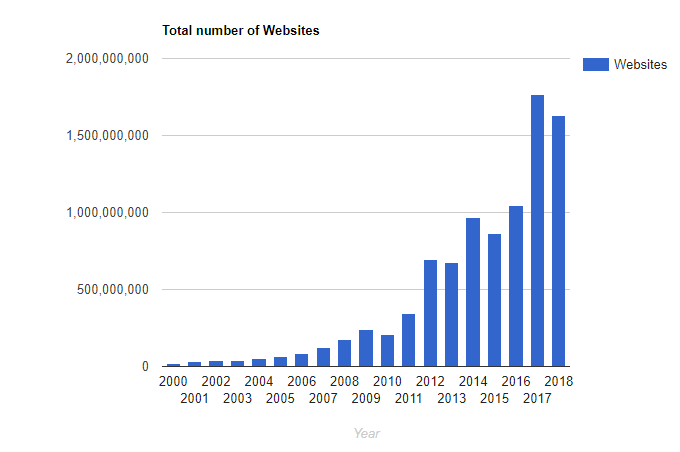
\includegraphics[width=\textwidth]{Images/numberOfWebsites.png}
    \caption{Total number of websites since 2000 (\cite{NumberofWebsites})}
    \label{Total number of websites since 2000}
\end{figure}
The majority of small businesses with a website are run by single individuals or small teams that do not necessarily have the time or resources to keep on top of their web traffic and potential attacks. The proposed application needs to account for the fact that these people will likely not have enough time to go through log files given their size. They also may not have the budget to buy solutions. It should be noted that a lot of web hosts do have automatic attack detection systems in place, as these are normally included in the cost of web hosting packages. However, many web hosts run a large number of servers, each of which often has a large volume of accounts. This can be seen in a recent article about cPanel's licensing update: Ryan Gray notes that 100 accounts in the early 2000s was a high number for one server, however now it is normal (\cite{cPanelArticle}). Due to their being more than one account on a server data would be aggregated to provide a overview of the server, therefore making some attacks harder to identify.

There are lots of different types of attack that can occur on a website. Some are easier to detect than others, for example, low bandwidth attacks are harder to detect. This was noted in 2014 by the National Research Council of Italy who say that "The problem is particularly challenging in virtue of the reduced amount of bandwidth generated by the attacks" (\cite{aiello2014line}). Therefore this implies that high bandwidth attacks are relatively easy to detect, so the focus of this dissertation will be to detect low bandwidth attacks and some other common attacks on websites that shall be discussed later. The findings will then be presented not to the server owner, but to the website owner so that they can be more informed about what is happening on their website.

The idea for this project came from when my own business website was attacked. I was fully prepared for a DDOS attack, however I found that there was an IP coming onto my site around 20 times in a minute that would then go away for a number of hours only to return some time later. The only way that I was able to detect this attack was by reading through that month's log file, which contained a few thousand lines of website logs, and comparing this to spikes in the server load. I felt that it would be helpful if there was a program to analyse the data. The only solutions out there were for large corporations, there wasn't anything for individual sites. There are also websites that monitor for suspicious IP addresses, for example https://www.abuseipdb.com/, however, as these would not take a server log file, you would need to input IP addresses one by one. Also, due to the fact the information is readily available online, the attackers know when they have been identified as a suspicious IP address and can easily change their IP address. Therefore there is a need for a solution that relies upon that background data but doesn't reveal what is known about an IP address. 

There is a vast amount of data in log files, although there are many limitations of the data held in these log files. They will record IP addresses however they can not record the location of those IP addresses. While there are tools such as google analytics that provide very detailed data on visitors to the site, these tools automatically filter out bots and do not show activity if the user generates an error. Another limitation of the log file comes from looking at the user agent field, whilst this records whether it is a bot, for example, google bot, this can be easily faked, and the log file cannot detect a fake google bot. Therefore, a fake google bot is a common form of attack (\cite{algiryage2018distinguishing}), due to the fact that the server cannot verify that it is a google bot.

The program will need to be easy to use for a non-expert website owner. Most website owners are computer literate however may not know how to access or analyse this type of data. Many website owners use content management systems (CMS). WordPress already has a lot of plugins available for security, and while these do a good job at blocking attacks in real-time and preventing invalid logins, they are not able to look at data over longer periods. The program aims to be compatible with all websites but due to the popularity of CMSs and wide variety of attack types, even websites that don't run a CMS  because of their market dominance (at time of writing, about 60\% of websites use WordPress (\cite{IsItWP})), may encounter these attacks without being aware.

\section{Proposed Work}
\label{proposed}
The work proposed is to write a piece of software, that will aid website management and detect traffic patterns that may take the form of a malicious attack. The finished software should also should include a database to store some data. During the main body of research I will debate and justify a type of software for writing the software. As part of the project I will also research and appropriate the most fitting database management system to handle my database storage. 

The literature review will include a critical analysis on current technologies to detect a variety attacks. This literature will help guide the development of the software by illuminating the gaps that exist in current technology. I will also look at whether network architecture can help to stop potential attacks. For example, services such as CloudFlare use an 'Anycast' network, wherein every server on the network has the same IP address, so that when a DDOS attack occurs they can spread the attack over many servers. The attacker cannot tell that they are not all going to the same server (\cite{CloudFlare}). CloudFlare could offer solutions to detect low bandwidth attacks as well.

I intend to develop the software using agile techniques. In other words, rather than fully writing the software first and then testing it, the software will be tested as throughout the development process. This will help to make the development time shorter as errors in the code will be fixed before the next stage of the software is written. 

\section{Aims and Objectives}
For this project I will have several aims and objectives.
\subsection{Aims}
\begin{enumerate}
    \item Develop a system that is able to identify different types of website traffic.
\end{enumerate}

\subsection{Objectives}
\begin{enumerate}
    \item Carry out a literature review and produce requirements documentation
    \begin{enumerate}
        \item Review of common attack techniques and how difficult or easy they are to detect.
        \item Review literature on how to present information to users on website data.
    \end{enumerate}
    \item Review of current protection that is available and how much data these programs release to the end user.
    \begin{enumerate}
        \item Look for attack prevention solutions for CMSs.
        \item Look for the reliability and ease of use for current attack prevention solutions.
    \end{enumerate}
    \item Produce relevant system documentation.
    \begin{enumerate}
        \item Produce relevant class diagram.
        \item Produce relevant Entity Relationship Diagrams (using crow's feet notation). 
        \item Produce relevant state transition diagram for interesting behaviour.
    \end{enumerate}
    \item Evaluate the project after completion.
    \begin{enumerate}
        \item Carry out a detailed test plan on the product.
        \item Check for usability with non-technical users.
    \end{enumerate}
    \item Abstract and introduction.
\end{enumerate}

\section{Skills}
For this project I will need several skills that I either already have and will develop or new skills that I will need to learn. Where I do not have the skill required I will consult learning tutorials and online literature in order to increase my knowledge. 

This project will require both networking and program skills. The networking skills will be important to ensure that I understand what the IP information tells us. This will need to be fed into the Java program in a way that is easy for the user to understand, and is not too big O complex due to the potential size of the data that could be submitted. 
\begin{enumerate}
\item Java 
\begin{enumerate}
    \item Java will form the main component of the project. I will therefore need to understand Java to a high enough standard to implement the program. Due to the complexities of the program using the right data structures to enable a quick response will be key to the program. 
    \item The majority of my modules have involved the use of Java. Even the modules that did not contain Java as a programming language helped me to develop a conceptual understanding of programming due to the concepts being similar across the board.
\end{enumerate}
\item SQL
\begin{enumerate}
    \item The main data for the project will be stored in a database, therefore it will be necessary to ensure that my SQL skills are up to scratch in order to store the data correctly and then the retrieval of the correct information will be crucial for this project. Some of the SQL queries may be complex in nature, for example nested queries may be needed.
    \item The module that most helped with SQL was the 'Relational Database' module, which covered the foundation of SQL databases, however SQL databases have also been used in the web modules and with Java in the 'Software Engineering Practice' module. \end{enumerate}
\item Networking Knowledge
\begin{enumerate}
    \item I have a basic understanding of networking and how networks work. I will need to learn how to apply this knowledge to detect attacks.
    \item I have gained some networking knowledge in the 'Computer Networks' module. 
    \item The majority of my working knowledge of networks, particularly the internet, came from my placement year, as I had to work with a variety of different websites and provide solutions to stop attacks. Nonetheless, my networking knowledge in identifying attacks is still limited and will need to be improved. 
\end{enumerate}
\item Time Management Skills
\begin{enumerate}
    \item As this is the largest project that I will work on during my undergraduate degree, I will need to manage my time well to ensure that I can get the work done and keep up with the other modules that I am taking this year. 
    \item I learnt a lot of time management skills in the 'Software Engineering' practical module. I will further develop these by asking my supervisor for advice early on and by researching time management techniques that work well for dissertation-style projects.
\end{enumerate}
\end{enumerate}

\section{Resources}

\subsection{Hardware}
\begin{enumerate}
    \item A PC - to write the software on.
\end{enumerate}
\subsection{Software}
\begin{enumerate}
    \item LAMP stack - a LAMP stack is needed to run websites on.
    \item Log files in the extended format
\end{enumerate}

\section{Structure and Contents of the Report}
\subsection{Report Structure}
\begin{enumerate} [topsep=0pt,itemsep=-0ex,partopsep=1ex,parsep=1pt,leftmargin=7ex,label=CH.\arabic*]
     \item Introduction
     \item Review of current detection methods for low bandwidth attacks
     \item Review of current detection methods for other types of attacks
     \item Tools and packages 
     \item Requirements Specifications
     \item Testing
     \item conclusions
\end{enumerate}

\subsection{List of Appendices}
\begin{enumerate} [label=\Alph*)]
    \item Terms of Reference
    \item Ethics form
    \item Risk Assessment
    \item ERD
\end{enumerate}
\section{Marking Scheme: General Project }
\textbf{Overview}

\begin{enumerate} [topsep=0pt,itemsep=-0ex,partopsep=1ex,parsep=1pt,label=]
    \item Report: 60\%
\begin{enumerate}[topsep=0pt,itemsep=-1ex,partopsep=1ex,parsep=1ex,label=]
\item Abstract \& Introduction 	5\%
\item Analysis 			30\%
\item Synthesis 			30\%
\item  Evaluation \& Conclusions 	30\%
\item Presentation 			5\%
\end{enumerate}
\item Product 30\%
\begin{enumerate}[topsep=0pt,itemsep=-1ex,partopsep=1ex,parsep=1ex,label=]
\item Fitness for Purpose 		50\%
\item Build Quality 			50\%
\end{enumerate}
\item Viva 10\%
\end{enumerate}

\clearpage

\section{Project Plan}
\noindent
\rotatebox{90}{%!TeX root=TermsOfReference.tex

% A lot of the settings here are tuned to fit a landscape gantt chart into
% an A4 piece of paper.
\begin{ganttchart}[
time slot format=little-endian,
calendar week text=\currentweek,
x unit=2.4pt,
y unit chart=14pt,
y unit title=12pt,
title label font=\scriptsize,
bar top shift=.15,
bar height=0.7,
milestone label font = \small,
group label font = {\tiny\bfseries},
group inline label node/.append style=centered,
hgrid=true,vgrid={*6{draw=none},dotted},
region/.style={inline,group peaks width=2,
  group peaks height=0.25, group height=0.5,
  group top shift=0.2 ,group/.append style={fill=#1}},
milestone left shift=0,
milestone right shift=1,
ms/.style={inline,
    milestone inline label node/.append style={#1=0pt}}
]{11/9/19}{18/05/20} %<- Dates Gantt Chart runs from and to

\gantttitlecalendar{year,month,week=1}\\
% Highlight Smesters and Vactions
\ganttgroup[region=blue!10]{Sem 1}{23/9/19}{20/12/19}
\ganttgroup[region=red!50]{Christmas}{20/12/17}{1/1/18}
\ganttgroup[region=blue!50]{Sem 2}{15/1/20}{23/3/20}
\ganttgroup[region=green!25]{Easter}{26/3/20}{13/4/20}
\ganttgroup[region=blue!50]{Sem 2}{16/04/20}{27/04/20}\\

% Project Deadlines (from the slides)
\ganttmilestone[]{TOR}{28/10/19}
\ganttmilestone[ms=left]{\bfseries TOR}{28/10/19}
\ganttmilestone[ms=right]{Draft Analysis}{6/12/19}
\ganttmilestone[ms=left]{Submit}{30/4/20}
\ganttnewline[thick]

% --Tasks go here
% put in a title, a start date, end date...
\ganttbar{TOR}{23/9/19}{21/10/19}
\ganttbar[inline]{\emph{revise}}{25/10/19}{10/11/19}\\
\ganttbar{Analysis}{18/9/19}{24/11/19}\\
\ganttbar{Design}{31/10/19}{17/1/20}\\
\ganttbar{Build}{17/1/20}{17/2/20}\\
\ganttbar{Test}{20/2/20}{16/3/20}\\
\ganttmilestone[ms=right]{Build complete}{18/2/20}
\end{ganttchart}
} %<- note use of \input{} not \include{}
\chapter{Ethics Form}
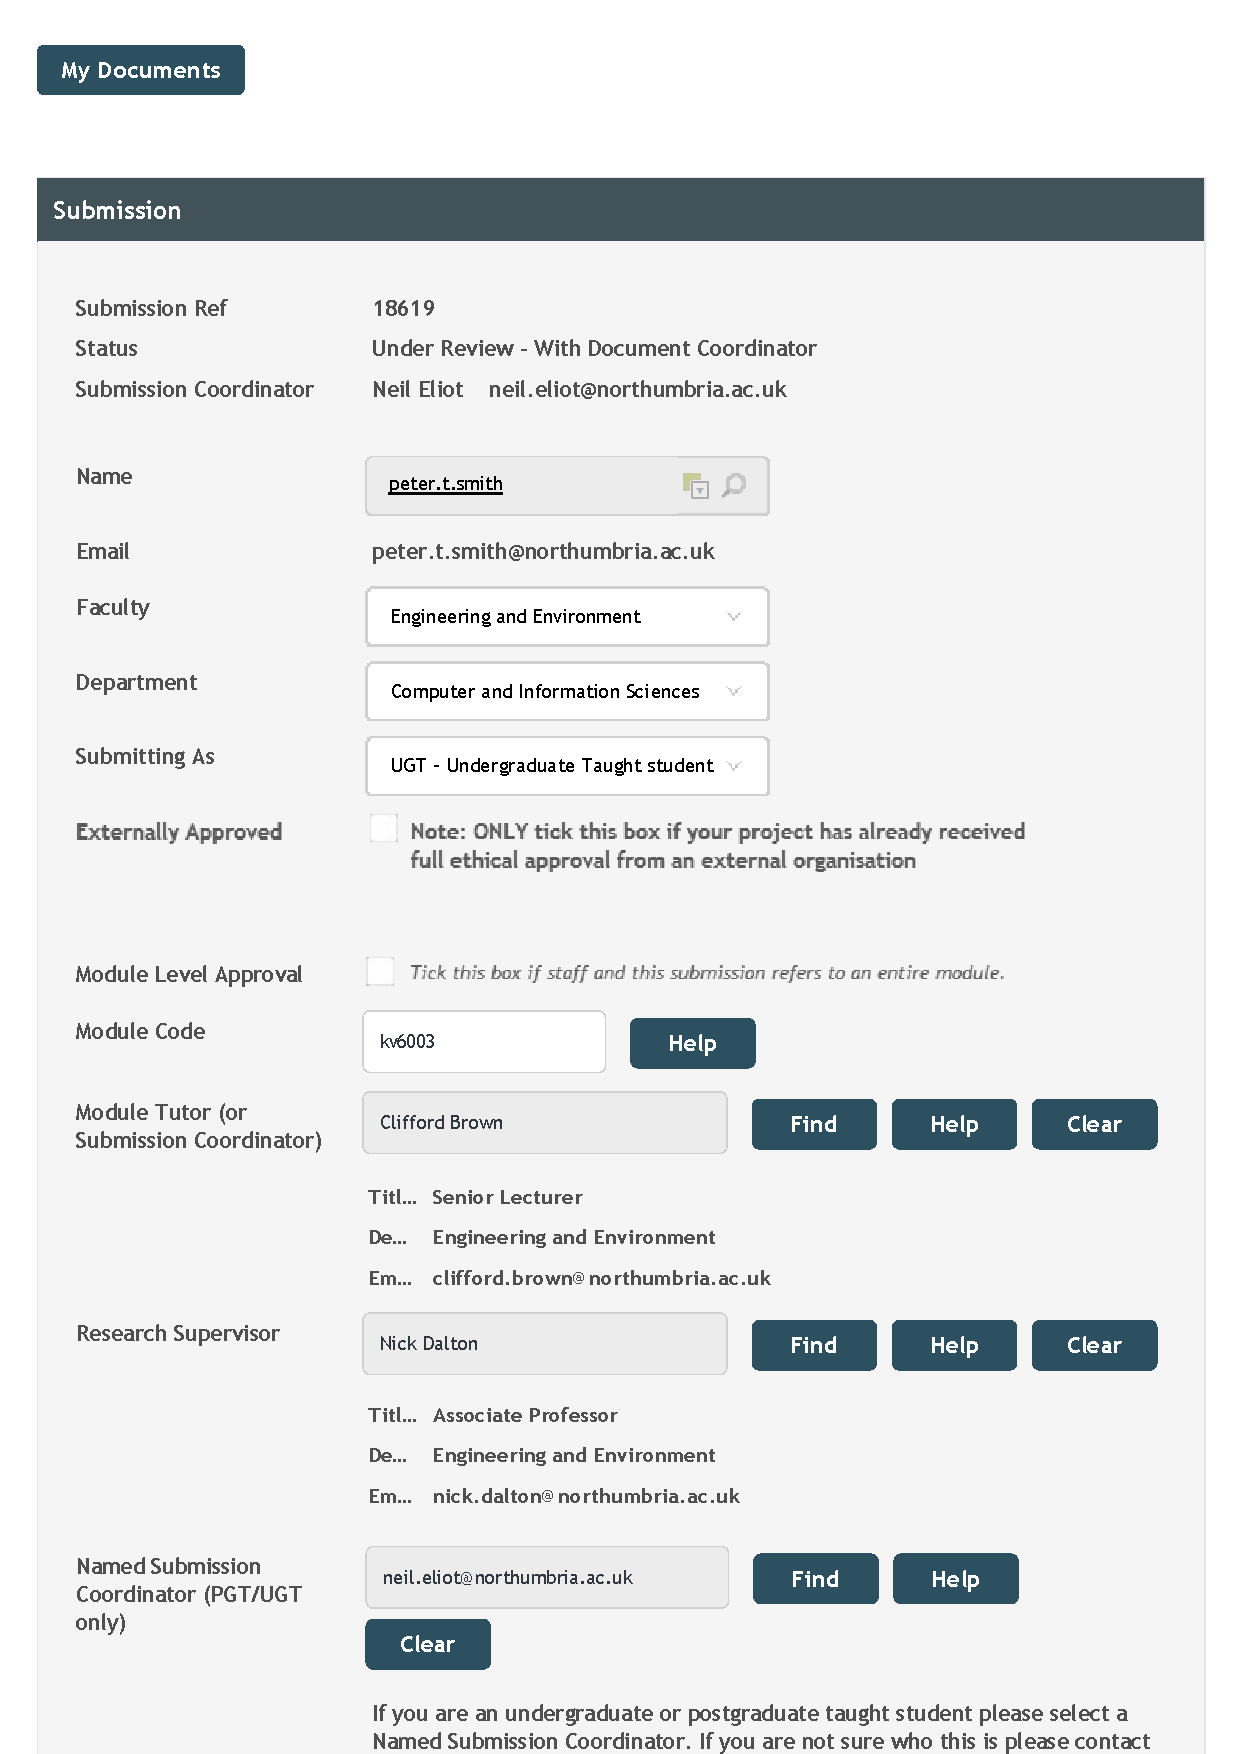
\includepdf[pages=-]{Apdenix/TermsOfReference/ResearchEthics18619.pdf}
\chapter{Participant Information Sheet}
%!TeX root=Dissertation.tex

\section{What is the purpose of this study?}
I have developed a small application to aid website owners to detect attacks on their website. This study aims to look at whether the software is usable for website owners. It is important to find out if website owners can use the software and understand the output of the data. I am conducting this study as part of my degree at Northumbria University. 
\section{Why have I been invited?}
You have invited to take part in this study as you are website owner or, you have the technical knowledge in web technology. 
\section{Do I have to take part?}
You do not have to take part in the study, you can stop at anytime. I am giving you this Participant Information Sheet to allow you to make an informed decision. You are fully able to decide whether or not you want to take part. 

\section{What will happen if I take part?}
You will be sat in front of a computer for about twenty minutes and will be asked to perform various tasks within the software. Your actions and comments will be captured using a screen recording software, you will be asked to think aloud and explain the reasons behind your actions on the software as well as what you are trying to achieve. After you have completed the task, you will be asked some general questions about your experience of using the software, this will ensure we get the same data from each participant. Your name will not be recorded on any information sheet or during the screen recording. The consent form that you will sign will not be stored with other data. On the questionnaire you will be given an I.D number which will be used to identify your recording so that we can check your questionnaire answers along with your recording. 
\section{How will my data stored and how long will it be stored for?}
Your paper consent form will be virtualised immediately upon completion and the original will be destroyed. The questionnaires will be completed online and the data will be retrieved from the online system, once all data is collected it will be deleted from the online system and stored in a password protected document on the university protected U-Drive. The videos will be stored on the university U-Drive and be destroyed after the work has been marked.  All data will be handled in accordance with the Data Protection Act (2018).
\section{What categories of personal data will be collected and processed in this study?}
Your name will be collected so that we can ensure we have your informed consent, as part of the data collection process we will be required to record your voice, this enables us to understand what users are thinking when using our software. 
\section{What is the legal basis for processing data?}
Based on the nature of the study, the data will be collected in accordance to Article 6(1)(e) "processing is necessary for the performance of a task carried out in the public interest". This study will collect a recording of your voice, due to this being sensitive personal data we will also be collecting data in accordance with Article 9 (2)(j) “processing is necessary for scientific and historical research purposes".
\section{Who are the recipients or categories of recipients of personal data, if any?}
No other external party will have access to the data provided during this study.
\section{What will happen to the results of the study and could personal data collected be used in future research?}
Once the dissertation has been marked, all personal data is deleted, any findings may be referenced in future research and the dissertation may be published.
\section{Who is Organizing and Funding the Study?}
This study is organised by Northumbria University. 
\section{Who has reviewed this study?}
The research project, submission reference 18619 has been approved in Northumbria University’s Ethics Online system. It has been reviewed in order to safeguard your interests, and have granted approval to conduct the study.
\section{What are my rights as a participant in this study?}
As a participant, you have the right to access a copy of the information collated in their personal data (to request access participants are required to submit a Subject Access Request); this can be done through email. If the participants notices that there is innacurate documentation of their personal data they have the right to request this to be corrected. You are also informed that if you are dissatisfied with the University’s processing of personal data, you have the right to complain to the Information Commissioner’s Office. 
\bigskip
\begin{center}\textbf{
    Contact for further information: }
    
Researcher Name: Peter Smith
Researcher email: peter.t.smith@northumbria.ac.uk
 
Supervisor: Nick Dalton 
Supervisor email: nick.dalton@northumbria.ac.uk

Second Marker: Neil Elliot
Second Marker email: neil.elliot@northumbria.ac.uk

Name and contact details of the Records and Information Officer at Northumbria University: Duncan James (dp.officer@northumbria.ac.uk). 

You can find out more about how we use your information at: www.northumbria.ac.uk/about-us/leadership-governance/vice-chancellors-office/legal-services-team/gdpr/gdpr---privacy-notices/ 
or by contacting a member of the research team

\end{center}
\chapter{Log file example} \label{Log file example}
\begin{figure}[H] 
    \centering
    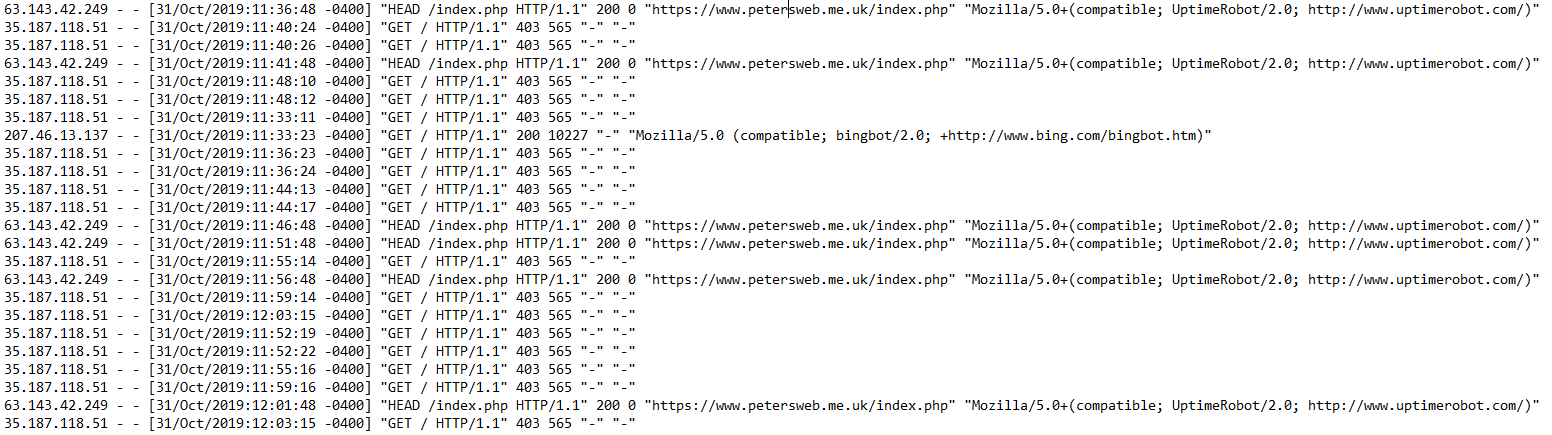
\includegraphics[width=170mm]{Apdenix/DodgyIPs.PNG}
    \caption{Log file example}
    \label{fig:my_label}
\end{figure}
\chapter{MOSCOW} \label{Moscow}
%!TeX root=Dissertation.tex

\section{Functional Requirements and Justification}
\textbf{Must}
\begin{enumerate}
    \item Allow users to analyse their website access logs.
    \begin{itemize}
        \item Users need to be able to import a large data set of website access logs, maybe a few months at a time to look for trends.
    \end{itemize}
    \item Allow users to access and view the data from their access logs.
    \begin{itemize}
        \item Users need to be able to interact with the data within the data set allowing them to make informed decisions on the data.
    \end{itemize}
    \item Use some kind of learning loop.
    \begin{itemize}
        \item Users may submit small data sets to analyse and the software needs to be able to use historical data to calculate risk. This approach could be done with the use of statistical analysis or by the use of an AI through fuzzy logic or computer learning.
    \end{itemize}
    \item Allow a admin to update known IP address'.
    \begin{itemize}
        \item An admin user needs to be able to add or remove a benign IP address' for services like google and Bing bots.
    \end{itemize}
    \item Be able to read log files.
    \begin{itemize}
        \item This will enable the detection of incoming attacks.
    \end{itemize}
        \item Allow data to be stored on an appropriate database
    \begin{itemize}
        \item For example  No SQL (MongoDB), SQL (Microsoft access)
    \end{itemize}
        \item Allow data to be stored securely in a database.
    \begin{itemize}
        \item The data that is collected needs to be stored securely in a database for future use.
    \end{itemize}
    \item Detect attacks
    \begin{itemize}
        \item The software must be able to detect a wide variety of attacks that can occur on web servers
    \end{itemize}
\end{enumerate}

\textbf{Should}
\begin{itemize}
    \item Allow users to filter data on data and time.
    \begin{itemize}
        \item Users may know a time-frame for an attack, therefore they may need to be able to narrow data down to this window.
    \end{itemize}
\end{itemize}
\textbf{Could}
\begin{itemize}
\item Be able to read log files that are in different formats.
    \begin{itemize}
        \item Consider the use of the following server types: Nginx, ISS.
    \end{itemize}
    \item Consider API integration.
    \begin{itemize}
        \item GOIPs, Abuse IPs.
    \end{itemize}
    \item Allow for concurrency in the database.
    \begin{itemize}
        \item If the software is developed further then there may be occasions when concurrency is needed within the database
    \end{itemize}
    
    \end{itemize}
\textbf{Won't}
\begin{itemize}
    \item Process the data on the server
    \begin{itemize}
        \item The only data that will be processed on the server will be the normal login or website traffic. The calculations of the formula will be processed on the PC of the person analyzing the data.
    \end{itemize}
    \item Automate the blocking of IP address' 
    \begin{itemize}
        \item Users need to maintain control of their own data, so if the program blocked IP addresses the users would not be in control. In addition to this there are a number or control panels (CPanel, plesk and custom panels) that would require custom APIs.
    \end{itemize}
\end{itemize}

\section{Non-Functional Requirements and Justification}
\textbf{Must}
\begin{itemize}
    \item Be maintainable, with well structured, commented, and documented code
    \begin{itemize}
        \item Following good practice and coding standards as well as making use of JavaDoc commenting will allow for code to be understood with greater ease, allowing for simpler maintenance and expansion of the project. 
    \end{itemize}
    \item Be able to analyse large amounts of data without draining large amounts of computational resources.
    \begin{itemize}
        \item The code shall be written to be as computationally simple as possible using the BigO notation.
    \end{itemize}
\end{itemize}
\textbf{Should}
\begin{itemize}
    \item The user interface should be aesthetically pleasing. 
    \begin{itemize}
        \item The design of the application should be easy on the eye, therefore making it easier to use.
    \end{itemize}
\end{itemize}
\textbf{Could}

\begin{itemize}
    \item Use Java for programming or find and alternative 
    \begin{itemize}
        \item Alternatives could include Python, C, PHP 
    \end{itemize}
    \item Consider making the upload facility flexible.
    \begin{itemize}
        \item There are different types of web-servers that can be used
    \end{itemize}
\end{itemize}
\textbf{Won't}\\
N/A
\chapter{Graph data} \label{Graph data}
\begin{figure}[H] \label{Log file example}
    \centering
    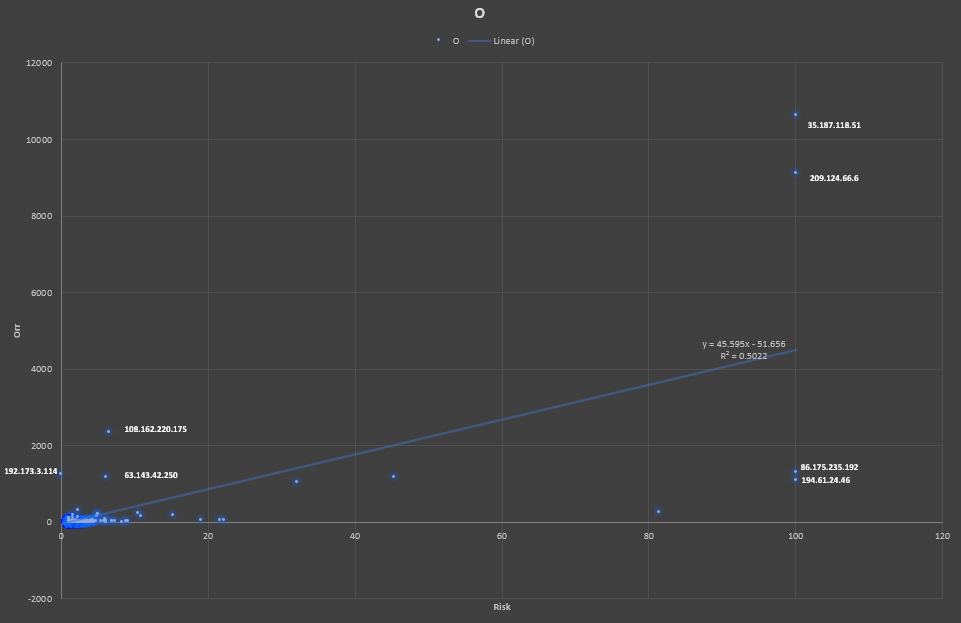
\includegraphics[width=170mm]{Apdenix/Graphdata.png}
    \caption{Log file example}
    \label{fig:my_label}
\end{figure}
\chapter{Formula Weights}
\section{Formula Weights (V.1)} \label{Weights}


The following weights are proposed for initial testing.

\begin{table}[H]
\begin{tabular}{ll}
Response Code & Weights \\
400           & +0.5    \\
401           & +5.0    \\
404           & +1.0 \\
403           & +2.0    \\
429           & +2.0    \\
500           & +0.2    \\
200           & -1.0   
\end{tabular}
\end{table}

If the URL contains 'Wp-Admin' then we shall apply an additional 3 to the risk related factor. If the URL contains 'login' in any case format an application of an additional 2 will be added to the risk factor. If the server responds with no data we shall apply an additional risk factor of 6.
\chapter{The Formula} \label{code}
\section{Code for formula}

%Python code highlighting
\label{Formula code}
\begin{lstlisting}[language=Java, caption=Formula code] 

	public double risk(String ip, DataStore dataStore, String countryCode) {
		double risk = 0;
		Database database = new Database();
		if (!database.knownBots(ip).equals("n/a")) {
			return risk;
		}
		double orrcancesOfipLog = Math
				.log(dataStore.getOrrcancesOfip().get(ip));
		orrcancesOfipLog = orrcancesOfipLog==0.00 ? 00.1 : orrcancesOfipLog;
		double countryRisk = database.countryRisk(countryCode); 
		double responseRisk = 0;
		double requestRisk = 0;
		for (Hits h : dataStore.getHits()) {
			if (h.getiPaddr().equals(ip)) {
				switch (h.getResponse()) {
				case 400:
					responseRisk += 0.5;
					break;
				case 401:
					responseRisk += 5;
					break;
				case 403:
					responseRisk += 2;
					break;
				case 404:
					responseRisk += 1;
					break;
				case 429:
					responseRisk += +2;
					break;
				case 500:
					responseRisk += 0.2;
					break;
				case 200:
					responseRisk -= 1;
					break;
				}
				if (containIgnoreCase(h.getRequest(), "wp-admin")) {
					requestRisk += 3;
				}
				if (containIgnoreCase(h.getRequest(), "login")) {
					requestRisk += 2;
				}
				if (h.getSize() == 0) {
					responseRisk = +6;
				}
			}

		}
		risk = (orrcancesOfipLog * 0.6) + ((requestRisk+responseRisk)*0.3) + (countryRisk * 0.1);
		if (risk > 100) {
			return 100;
		} else if (risk < 1) {
			return 1;
		} else {
			return risk;
		}
	}
\end{lstlisting}

\chapter{User Interface Screenshots} \label{User Interface Screenshots}
\begin{figure}[H]
  \begin{subfigure}[b]{\textwidth}
    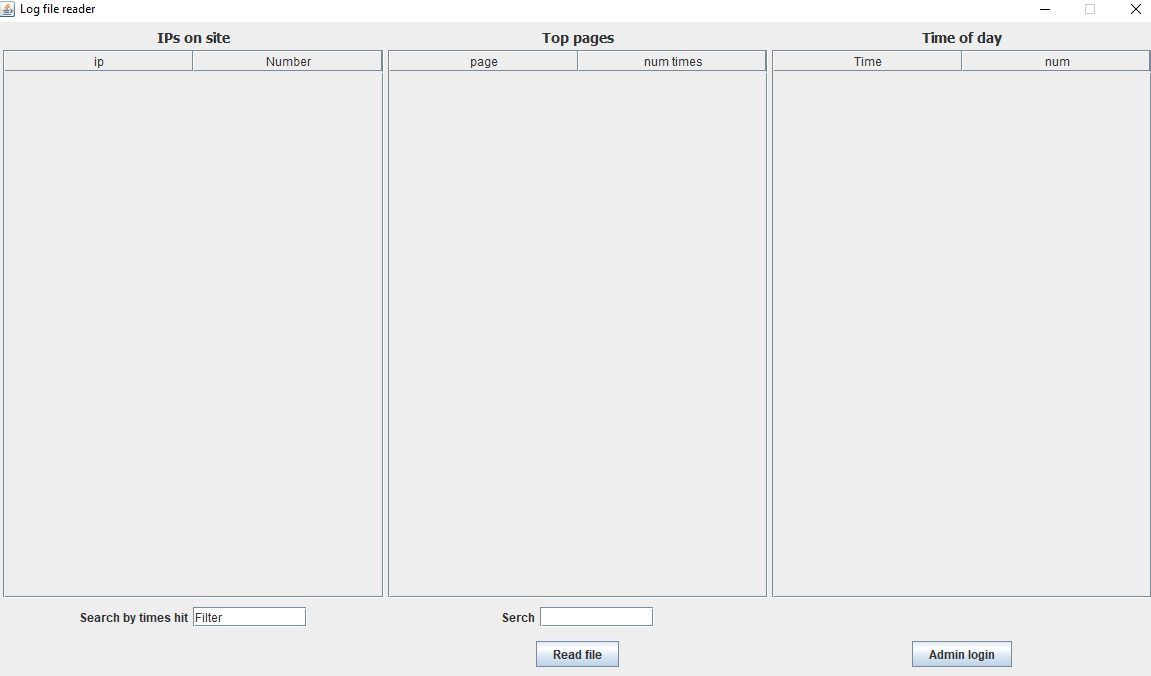
\includegraphics[width=\textwidth]{Apdenix/ui1.PNG}
    \caption{UI (1)}
    \label{fig:1}
  \end{subfigure}
  %
  \begin{subfigure}[b]{\textwidth}
    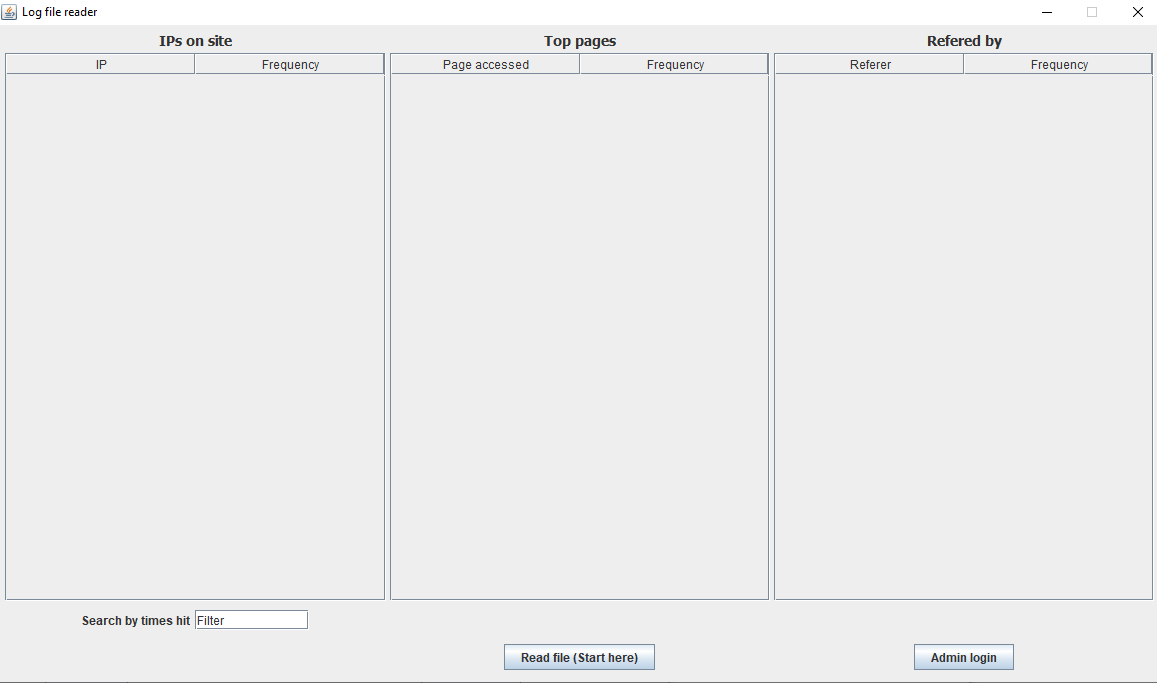
\includegraphics[width=\textwidth]{Apdenix/ui2.PNG}
    \caption{UI (2)}
    \label{fig:2}
  \end{subfigure}
  \caption{Screen shots of the UI's before and after changes}
\end{figure}

\chapter{Log Book}
\includepdf[pages=-]{Apdenix/logbook.pdf}
\end{document}
